% Options for packages loaded elsewhere
\PassOptionsToPackage{unicode}{hyperref}
\PassOptionsToPackage{hyphens}{url}
%
\documentclass[
]{book}
\usepackage{amsmath,amssymb}
\usepackage{lmodern}
\usepackage{ifxetex,ifluatex}
\ifnum 0\ifxetex 1\fi\ifluatex 1\fi=0 % if pdftex
  \usepackage[T1]{fontenc}
  \usepackage[utf8]{inputenc}
  \usepackage{textcomp} % provide euro and other symbols
\else % if luatex or xetex
  \usepackage{unicode-math}
  \defaultfontfeatures{Scale=MatchLowercase}
  \defaultfontfeatures[\rmfamily]{Ligatures=TeX,Scale=1}
\fi
% Use upquote if available, for straight quotes in verbatim environments
\IfFileExists{upquote.sty}{\usepackage{upquote}}{}
\IfFileExists{microtype.sty}{% use microtype if available
  \usepackage[]{microtype}
  \UseMicrotypeSet[protrusion]{basicmath} % disable protrusion for tt fonts
}{}
\makeatletter
\@ifundefined{KOMAClassName}{% if non-KOMA class
  \IfFileExists{parskip.sty}{%
    \usepackage{parskip}
  }{% else
    \setlength{\parindent}{0pt}
    \setlength{\parskip}{6pt plus 2pt minus 1pt}}
}{% if KOMA class
  \KOMAoptions{parskip=half}}
\makeatother
\usepackage{xcolor}
\IfFileExists{xurl.sty}{\usepackage{xurl}}{} % add URL line breaks if available
\IfFileExists{bookmark.sty}{\usepackage{bookmark}}{\usepackage{hyperref}}
\hypersetup{
  pdftitle={What makes an R-package popular?},
  pdfauthor={Yiwen Zhang},
  hidelinks,
  pdfcreator={LaTeX via pandoc}}
\urlstyle{same} % disable monospaced font for URLs
\usepackage{longtable,booktabs,array}
\usepackage{calc} % for calculating minipage widths
% Correct order of tables after \paragraph or \subparagraph
\usepackage{etoolbox}
\makeatletter
\patchcmd\longtable{\par}{\if@noskipsec\mbox{}\fi\par}{}{}
\makeatother
% Allow footnotes in longtable head/foot
\IfFileExists{footnotehyper.sty}{\usepackage{footnotehyper}}{\usepackage{footnote}}
\makesavenoteenv{longtable}
\usepackage{graphicx}
\makeatletter
\def\maxwidth{\ifdim\Gin@nat@width>\linewidth\linewidth\else\Gin@nat@width\fi}
\def\maxheight{\ifdim\Gin@nat@height>\textheight\textheight\else\Gin@nat@height\fi}
\makeatother
% Scale images if necessary, so that they will not overflow the page
% margins by default, and it is still possible to overwrite the defaults
% using explicit options in \includegraphics[width, height, ...]{}
\setkeys{Gin}{width=\maxwidth,height=\maxheight,keepaspectratio}
% Set default figure placement to htbp
\makeatletter
\def\fps@figure{htbp}
\makeatother
\setlength{\emergencystretch}{3em} % prevent overfull lines
\providecommand{\tightlist}{%
  \setlength{\itemsep}{0pt}\setlength{\parskip}{0pt}}
\setcounter{secnumdepth}{5}
\usepackage{booktabs}
\usepackage{amsthm}
\usepackage{bera}
\usepackage{tcolorbox}
\makeatletter
\def\thm@space@setup{%
  \thm@preskip=8pt plus 2pt minus 4pt
  \thm@postskip=\thm@preskip
}
\makeatother

\newenvironment{discovery}[1]{%
  \begin{tcolorbox}[colback=blue!30,colframe=blue!80!black]#1}{\end{tcolorbox}}
\usepackage{booktabs}
\usepackage{longtable}
\usepackage{array}
\usepackage{multirow}
\usepackage{wrapfig}
\usepackage{float}
\usepackage{colortbl}
\usepackage{pdflscape}
\usepackage{tabu}
\usepackage{threeparttable}
\usepackage{threeparttablex}
\usepackage[normalem]{ulem}
\usepackage{makecell}
\usepackage{xcolor}
\ifluatex
  \usepackage{selnolig}  % disable illegal ligatures
\fi
\usepackage[]{natbib}
\bibliographystyle{authoryear}

\title{What makes an R-package popular?}
\author{Yiwen Zhang}
\date{2021-06-14}

\begin{document}
\maketitle

{
\setcounter{tocdepth}{1}
\tableofcontents
}
\hypertarget{preface}{%
\chapter*{Preface}\label{preface}}
\addcontentsline{toc}{chapter}{Preface}

As an R user, have you ever thought about what kind of information is hidden behind the numbers of downloads for R and R-packages? Why would there be an abnormal download volume? When choosing which package to use, we likely often tend to use popular ones. But what kind of packages are popular? And what factors can be linked to the popularity of an R-package? I propose those are questions as those most R users will be curious about. Therefore, based on the existing findings, this report attempts to provide answers and directions of enquiry towards the above questions, by taking an exploratory data analysis approach.

This report is written as part of the ETC5543 research project, supervised by Drs Emi Tanaka and Hien Nguyen. Due to the limitations of my programming ability, I encountered some obstacles during this research. But this is also a very precious opportunity for me to cultivate my research thinking and improve my confidence in coding.

I would like to express my very great appreciation to Drs Emi Tanaka and Hien Nguyen for their valuable and constructive suggestions during the planning and development of this research work. As my supervisors, their patient guidance, enthusiastic encouragement and willingness to give their time so generously have been very much appreciated. And my special thanks are also extended to Drs Emi Tanaka and Hien Nguyen for their generous help on writing. I would like to also thank Professor Rob J Hyndman, for holding meetings every two weeks to give us recommendations.

I hope you enjoy your reading.

\hypertarget{abstract}{%
\chapter{Abstract}\label{abstract}}

This research seeks to analyze the popularity of R-packages and figure out the probably influential factors that drive such popularity. Data are closely related to social and economic activities in our daily life, so data mining and analysis can often be beneficial. This research focuses on R in this project, and aims to explore the popularity of R-packages from CRAN (the Comprehensive R Archive Network). To achieve this, it is assumed in this research that the download volume is a relatively reliable and simple measurement for the popularity of an R-packages, and two main parts of analysis has been carried out : one is to uncover the information behind the download count logs, the other is to explore the factors that can be linked to the download volume. The technical aspects that are applied in this research is largely compromise of R programs and scripts, together with some Python code on data scraping. By obtaining the daily and recent half year total download counts of 17,713 R-packages and R itself, this research analyzes pattern, characteristics, as well as the relationship between the release dates, update times, numbers of commits on Github (master or main branch), name lengths and alphabetical order of the names. Finally, this research also provides some description of the changes of R-user preferences on 1st April over the period of 2013 to 2021.

Results show that the daily downloads of R-packages have a strong weekly seasonality and unusual spikes caused by repeat downloads, updates or server test issue. The most stably popular R-packages over the period of 2017 to 2019 is related to JAVA dependency. We also found that an earlier release date is more likely to result in a higher download volume for R-packages. Similarly, update times and commits numbers on master (main) branch in Github repositories are also positively correlated with download volumes. However, the alphabetical order of R-package names contributes little to the download counts.

KEY WORDS : R-package popularity, CRAN download volume, Web scraping, Github API, EDA

\hypertarget{intro}{%
\chapter{Introduction}\label{intro}}

Data have penetrated into every industry and business field, has become an increasingly important factor of production and consumption in our lives. However, data must be processed to uncover the information within. For this reason many statistical tools have been produced, such as SPSS, Python, R and so on. In this project, we focus on the R language \citep{R-base}.

R is a programming language and environment for statistical computing and graphics, which can be extended easily via packages and provide an Open Source route to participation in statistical methodology. It is available as Free Software under the terms of the Free Software Foundation's GNU General Public License \citep{gnu}. R is one of the most popular statistical languages and has been ranked competitively, even among the general purpose programming languages \citep[peaking 8th in August 2020 in][]{tiobe}. The TIOBE Programming Community index aggregates several search engines to derive a metric of the popularity of a programming language. It is important to note, however, that programming languages ranked higher than R are mostly general purpose languages and therefore naturally have a larger user base.

Today, R is greatly enhanced by over 17,713 R-packages contributed by hundreds of developers all over the world. However, when R originally appeared in August of 1993 with its first official release in June of 1995 \citep{Ikaha1998}, the contributions were managed by only a small group of core developers. In April of 1997, the Comprehensive R Archive Network (CRAN) was established as the official R-packages repository, with 3 mirror sites. Now, the source repositories to install R-packages have expanded to Bioconductor, Gitlab, GitHub, R-Forge and \href{https://cran.r-project.org/mirmon_report.html}{106 CRAN mirrors in 49 regions}. Of all the CRAN mirrors, the daily download counts for each package is only readily available from the RStudio CRAN mirror. In this report, we will be focusing only on one CRAN mirror of RStudio, albeit it being the most popular one, for exploratory data analysis. Henceforth, all download counts of packages refer to the download from this RStudio CRAN mirror.

CRAN is a network of ftp and web servers around the world that store identical, up-to-date, versions of code and documentation for R \citep{CRAN}.

The most intuitive measurement of popularity is the total number of downloads, although it does not directly reflect the number of users, because it includes repeated downloads by the same user, updates and test downloads caused by the server. Briefly, some works concerning the reporting and interpretation of these download counts include: the R-package \texttt{adjustedcranlogs} \citep{adjustedcranlogs}, which attempts to correct for download inflation using a heuristic approach; the package \texttt{packageRank} \citep{packageRank}, which provides a way to compute the rank percentile for packages and filters invalid downloads, including small and medium size logs. There are also some packages such as \texttt{pkgsearch}\citep{pkgsearch} and \texttt{Visualize.CRAN.Downloads}\citep{VisualizeCRANDownloads} that provide some visualization methods to explore the package download trends or for convenient searching. More details are provided in Section 5.

Based on those initial works, researchers have started to study the popularity of R-packages from CRAN. We still assume in this project that, the download amount is a relatively reliable and simple measure of a R-package's popularity. The previous studies, the R-package \texttt{adjustedcranlogs}\citep{adjustedcranlogs} finds that there are spikes in downloads due to automatic re-downloads and package updates, and it also provides a method to remove these download logs. Some of the methods are function extensions based on previous packages, and some of their proposed methods are new functions, but generally speaking, they are more tool like, to help users explore the characteristics of package download logs from as many directions as possible.

As for us, the purpose of this project is to explore the download logs of R-packages on CRAN and to analyze the relationships between some probably influential factors, to help users and developers better understand the download patterns, and also figure out what could determine a R-package's popularity to some extent.

\begin{itemize}
\item
  A CRAN mirror is a website containing differently located servers, which aims to facilitate to quick and smooth access for people from different regions and countries. Each server is called a mirror \citep{cranmirror}.
\item
  CRAN task view aims to provide some guidance regarding which packages on CRAN are relevant for tasks related to a certain topic \citep{crantaskviews}.
\end{itemize}

\hypertarget{other-work}{%
\section{Other work}\label{other-work}}

\texttt{adjustedcranlogs}\citep{adjustedcranlogs} : In this tool, unusual download spikes are smoothed over and the upward download bias is removed stochastically by subtracting the minimum download count from a random sampling of packages; if this corrected download results in a negative value then this is adjusted to be zero.

\hypertarget{data}{%
\chapter{Data}\label{data}}

The main source of data used in this report is the download logs from the RStudio CRAN mirror site : \url{https://cran.rstudio.com/}. These log files are created for every instance of download of an R-package via the RStudio CRAN mirror, then these log files are processed, daily, into CSV files that contain the following variables with the name of header in brackets:

\begin{itemize}
\tightlist
\item
  Date (\texttt{date}),
\item
  Time in UTC time zone (\texttt{time}),
\item
  Size of the file in bytes (\texttt{size}),
\item
  Version of R used to download the package (\texttt{r\_version}),
\item
  Architecture type for R (i386 = 32 bit, x86\_64 = 64 bit) (\texttt{r\_arch}),
\item
  Operating System (darwin9.8.0 = mac, mingw32 = windows) (\texttt{r\_os}),
\item
  Package (\texttt{package}),
\item
  Country in two letter ISO country code (\texttt{country}), and
\item
  Anonymised daily unique id (\texttt{ip\_id}).
\end{itemize}

A similar log file is also created for every download of R from the RStudio CRAN mirror with the processed log file generating a CSV file that contains the same variables except \texttt{r\_arch} and \texttt{package}, and \texttt{r\_version} and \texttt{r\_os} are named as \texttt{version} and \texttt{os}. These CSV files are hosted at \url{http://cran-logs.rstudio.com/} and updated daily with data available from 1st October 2012.

The log files of a particular day is processed and compressed into a single CSV file of about 40 megabytes (file sizes of earlier years are much smaller due to lower number of download logs). As there are over 700,000 CSV files, a simple estimate of the size of the data is 28 terabytes - far exceeding typical portable hard drives which are 1-4 terabytes.

The summarised version of data, where the data show the total daily download counts for each package, is accessible using the \texttt{cranlogs} R-package. The \texttt{cranlogs} package accesses this summary data through the web application programming interface (API) maintained by r-hub \citep{rhub}.

\hypertarget{methods}{%
\chapter{Methods}\label{methods}}

In this project, we extracted R-package names from CRAN and obtained summary daily download logs of R-packages through the web Application Programming Interface (API) maintained by r-hub\citep{rhub}. We also collected release dates of R-packages through CRAN. In addition, we also tried to scrap the number of commits on master (main) branch in Github repositories for all of available R-packages. Then we conducted eight exploratory data analysis studies:

\begin{itemize}
\item
  we explored the daily downloads of all the packages on CRAN and figured out the number of R-packages occupied by different downloaded groups;
\item
  we analyzed the daily download trend of R itself and the found out the most popular version of R;
\item
  we compared the top 15 downloaded R-packages on CRAN, yearly, on 1st April. from 2013 to 2021, to see how user preference change;
\item
  we figured out the relationship between initial release dates and the total download counts over the most recent 6 month period. The reason for choosing the period of 6 months is : different R-packages are initially released in different time. If the comparison period is too long, it will be unfair to the R-packages released later. And if the period is too short, download data will be not enough to reflect some potential patterns or relationships;
\item
  we compared two closely related packages : \texttt{fable} and \texttt{forecast}, to see the difference between their MA (moving average) trends;
\item
  we studied how the number of commits on master (main) branches in Github repositories may influence the total download counts for the most recent 6 month period;
\item
  we explored the relationship between the number of updates for all of R-packages and their download counts;
\item
  we analyzed the name length patterns for both CRAN task view packages and all of R-packages on CRAN;
\item
  we explored how the alphabetical order of R-packages would related to the download counts and the statistic features (e.g.variance, median of the download counts).
\end{itemize}

\hypertarget{results}{%
\chapter{Results}\label{results}}

\hypertarget{daily-downloads-of-r-packages}{%
\section{Daily downloads of R-packages}\label{daily-downloads-of-r-packages}}

\begin{discovery}
\textbf{Finding 1}: There was unusual download activities in one day of
2014 and 2018.
\end{discovery}

In this first section, we studied the daily downloads of CRAN R-packages from 2012-10-01 to 2021-06-12. The data was obtained from the \texttt{cranlogs} package\citep{cranlogs}, which includes a summary of the download logs via the RStudio CRAN mirror. The daily download data for CRAN R-packages are available from 1st October 2012. Examination of this data showed two unusual observations in 2014 and 2018 as shown in Figure \ref{fig:unusual-spikes}. The one happening in 2014 was on 2014-11-17, Monday, while the other one happening in 2018 was on 2018-10-21, Sunday.



\begin{figure}

{\centering 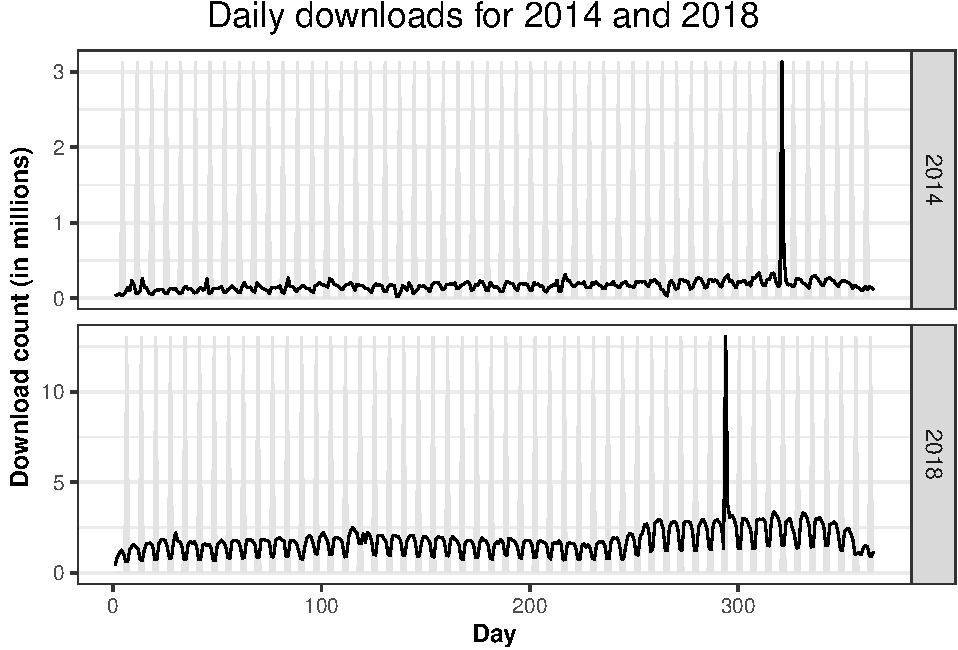
\includegraphics{figures/unusual-spikes-1} 

}

\caption{Unusual download spikes in 2014 and 2018.}\label{fig:unusual-spikes}
\end{figure}

When having a closer look into those two spikes, we firstly focused on the one on 2014-11-17. From Table \ref{tab:spike14count}, we could see that the downloads of top downloaded R-packages on this day differs little, indicating this spike is not due to a certain package.

\begin{table}

\caption{\label{tab:spike14count}The total downloads of each R-package on 2014-11-17}
\centering
\begin{tabular}[t]{l|r}
\hline
package & n\\
\hline
BayHaz & 767035\\
\hline
clhs & 660298\\
\hline
GPseq & 394840\\
\hline
OPI & 382518\\
\hline
YaleToolkit & 370513\\
\hline
survsim & 224994\\
\hline
BAT & 40592\\
\hline
Rcpp & 3509\\
\hline
ggplot2 & 3167\\
\hline
plyr & 3150\\
\hline
\end{tabular}
\end{table}

Table \ref{tab:spike14country} shows the downloads from different countries on 2014-11-17. It is obvious that \texttt{Indonesia} obtains much more downloads than any others.

\begin{table}

\caption{\label{tab:spike14country}The countries downloading from CRAN on 2014-11-17}
\centering
\begin{tabular}[t]{l|r}
\hline
country & n\\
\hline
ID & 2863576\\
\hline
US & 96336\\
\hline
CN & 32729\\
\hline
DE & 14548\\
\hline
FR & 11860\\
\hline
GB & 10491\\
\hline
IN & 8635\\
\hline
HK & 8090\\
\hline
BE & 7720\\
\hline
KR & 6794\\
\hline
\end{tabular}
\end{table}

Furthermore, we also checked IP addresses, displayed in Table \ref{tab:spike14ip}. Downloads from \texttt{ip3758} is much higher than others. So, it seems that most of the downloads are owing to one certain IP for the unusual spike in 2014.

\begin{table}

\caption{\label{tab:spike14ip}The IP addresses downloading from CRAN on 2014-11-17}
\centering
\begin{tabular}[t]{r|r}
\hline
ip\_id & n\\
\hline
3758 & 2863432\\
\hline
11536 & 6244\\
\hline
11725 & 5992\\
\hline
16385 & 5991\\
\hline
534 & 5986\\
\hline
3784 & 5983\\
\hline
18519 & 4511\\
\hline
80 & 2124\\
\hline
27 & 1892\\
\hline
464 & 1375\\
\hline
\end{tabular}
\end{table}

Next, we turned to the unusual spike in 2018. Table \ref{tab:spike18count} shows the downloads from \texttt{tidyverse} is much higher than others, with nearly three orders of magnitude.

\begin{table}

\caption{\label{tab:spike18count}The total downloads of each R-package on 2018-10-21}
\centering
\begin{tabular}[t]{l|r}
\hline
package & n\\
\hline
tidyverse & 11692582\\
\hline
Rcpp & 16263\\
\hline
stringi & 13981\\
\hline
rlang & 13796\\
\hline
ggplot2 & 13306\\
\hline
dplyr & 13081\\
\hline
glue & 12593\\
\hline
digest & 12302\\
\hline
stringr & 11505\\
\hline
fansi & 11275\\
\hline
\end{tabular}
\end{table}

As for country, from Table \ref{tab:spike18country}, we could know that \texttt{US} occupies the most part of downloads on that day.

\begin{table}

\caption{\label{tab:spike18country}The countries downloading from CRAN on 2018-10-21}
\centering
\begin{tabular}[t]{l|r}
\hline
country & n\\
\hline
US & 12140853\\
\hline
NA & 179847\\
\hline
GB & 76624\\
\hline
IN & 51502\\
\hline
CN & 46095\\
\hline
TR & 36590\\
\hline
AU & 35078\\
\hline
DE & 32837\\
\hline
CA & 31125\\
\hline
KR & 30469\\
\hline
\end{tabular}
\end{table}

Finally, the most interesting finding is on IP address, displayed in Table \ref{tab:spike18ip}. Several consecutive IPs have highly distinguished downloads. It seems that they are probably from the same individual, or caused by a server test issue, in such a short period of time.

\begin{table}

\caption{\label{tab:spike18ip}The IP addresses downloading from CRAN on 2018-10-21}
\centering
\begin{tabular}[t]{r|r}
\hline
ip\_id & n\\
\hline
266 & 3034720\\
\hline
263 & 2457383\\
\hline
655 & 2099321\\
\hline
264 & 1557640\\
\hline
267 & 1406876\\
\hline
265 & 1032535\\
\hline
2 & 179711\\
\hline
268 & 99932\\
\hline
112 & 34397\\
\hline
3296 & 17223\\
\hline
\end{tabular}
\end{table}

To sum up, we found that these two unusual spikes have one thing in common, that is, most of the downloads came from a specific country. The difference is that in 2014, a large number of downloads came from several different R-packages, while in 2018, they came from only one package \texttt{tidyverse}. In addition, in 2014, a large quantities of downloads came from one IP, while in 2018, they came from several consecutive IPs, At this point, it is guessed that they should come from the same individual, and it is very likely due to sever test issue, for it may be not necessary or reasonable for an individual to generate such a large amount downloads in one day.

\begin{discovery}
\textbf{Finding 2}: There are increasing numbers of downloads over time,
which can attests the growing number of R users.
\end{discovery}

Figure \ref{fig:download-over-time} shows the download trend of all R-packages on CRAN over a period pf time from 2012-10-01 to 2021-06-12, after fixing the unusual spikes mentioned above. There is an upward trend, with an increasing variance in download counts.



\begin{figure}

{\centering 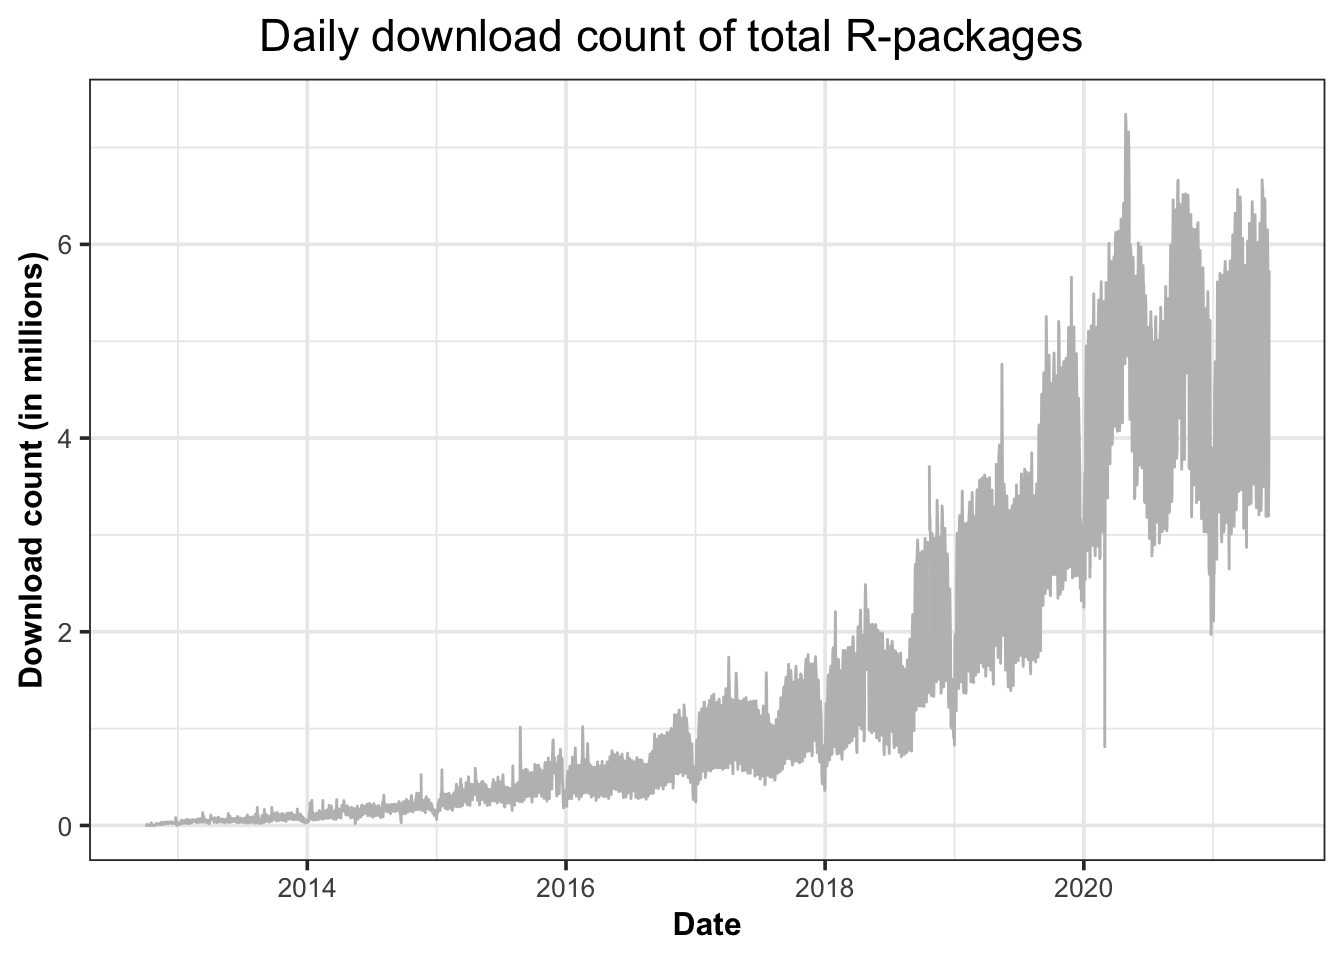
\includegraphics{figures/download-over-time-1} 

}

\caption{The download trend of all R-packages on CRAN from 2012-10-01 to 2021-06-12.}\label{fig:download-over-time}
\end{figure}

\begin{discovery}
\textbf{Finding 3}: Weekends have a lower downloads than weekdays.
\end{discovery}

To have a closer look at the weekly pattern, figure \ref{fig:total-trend} shows the daily downloads of all CRAN R-packages via the RStudio mirror, with the grey areas highlighting the weekend.

To be more specific, except for 2012 and 2013, the patterns of other years are very similar, with a strong weekly seasonality. To be more detailed, in 2012, the download logs showed an overall upward trend, which also reflected more and more users there after release of CRAN. In the following years, there is no obvious trend in download volume, but a strong seasonality, which indicates that in a week, the total downloads always increases first then decreases, and reaches the lowest on weekends. Although the pattern of 2013 is more volatile, it still conforms to that. We suppose that is because CRAN was only open for a short period of time in 2013, so the amount of download data is not adequate to show the weekly pattern very clearly. After 2016, the pattern of each year is quite consistent, for the total downloads have been increasing year by year. Back to weekly seasonality, people are more likely to download packages during weekdays, and rest on weekends. So, the trough of download curve always occurs on weekends. In addition, the lowest downloads across the year are always happening at the end of December or the beginning of January, probably due to the Christmas and New Year's holidays. Meanwhile, the downloads are on the rise from August to October, and from February to April, which covers the beginning of semesters for many universities around the world, a time when related students tend to download CRAN R-packages very often.



\begin{figure}

{\centering 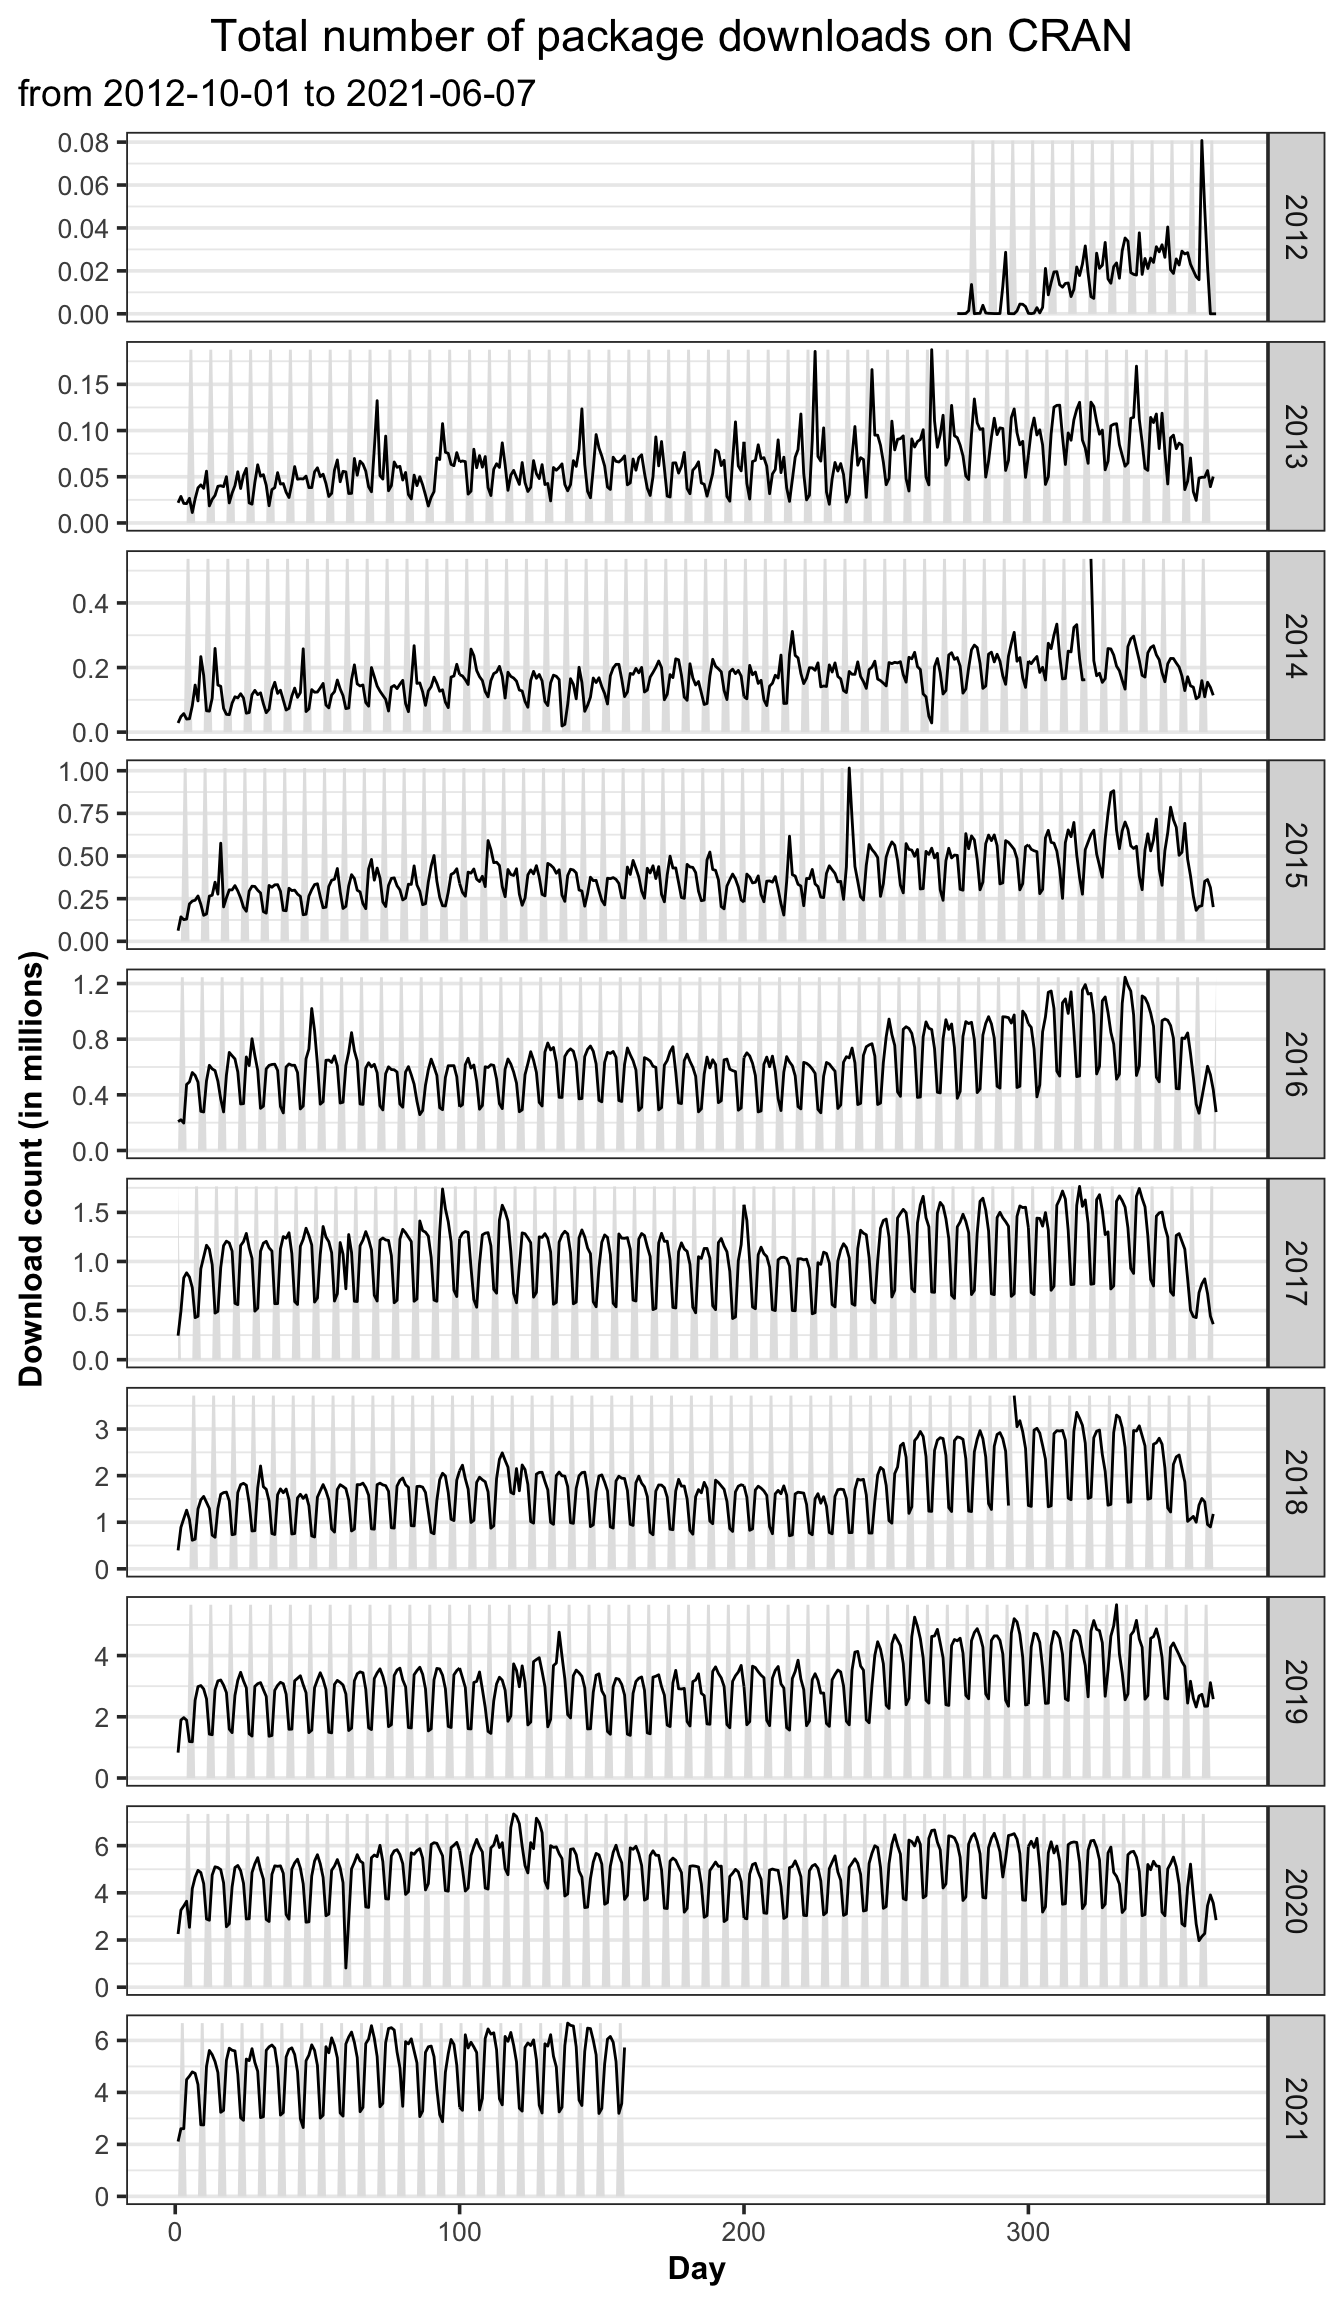
\includegraphics{figures/total-trend-1} 

}

\caption{The total downloads for all of R-packages on CRAN would decrease on weekends and increase during weekdays.}\label{fig:total-trend}
\end{figure}

As there are many fluctuations in daily download pattern, which is due to calendar effect and test server issue of CRAN mirror, an STL decomposition model explained in \citet{stl}, was applied, to smooth the curve for all of the R-packages in Figure \ref{fig:pkg-stl}.



\begin{figure}

{\centering 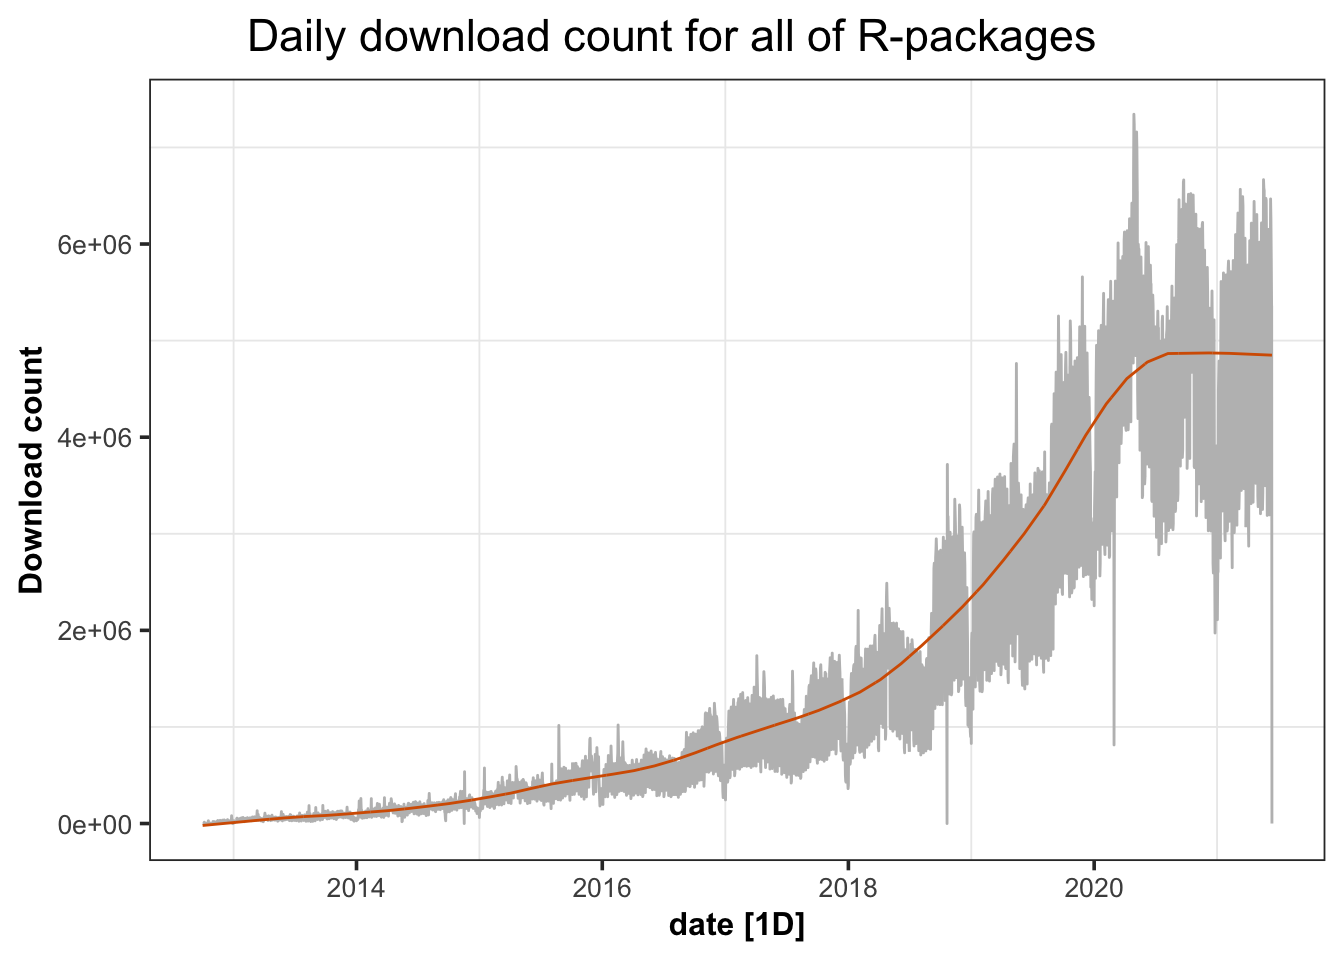
\includegraphics{figures/pkg-stl-1} 

}

\caption{The total downloads of all R-packages on CRAN after smoothing.}\label{fig:pkg-stl}
\end{figure}

Figure \ref{fig:weekend-vs-weekday} shows the distributions and the median of the downloads between weekday and weekends, which differ from each other a lot. The violin plots of weekends are wider and shorter, while those of weekdays are thinner and higher, on the contrary. That is because the total downloads on weekends are less than those in weekdays. In 2012, the median and interquartile range of download logs are not very distinguished between weekdays and weekends, for the data volume was not adequate at this time as mentioned before. But after 2013, the gap between the two has been becoming more and more obvious. The median downloads of working days are significantly higher than those of weekends, and the overall download volume is also significantly larger than that of weekends as well. Interestingly, the lower adjacent sometimes occurs on weekends, such as in year 2014, 2015, 2018, 2019 and 2021, while sometimes also in weekdays, such as in year 2012, 2013, 2016, 2017 and 2020.



\begin{figure}

{\centering 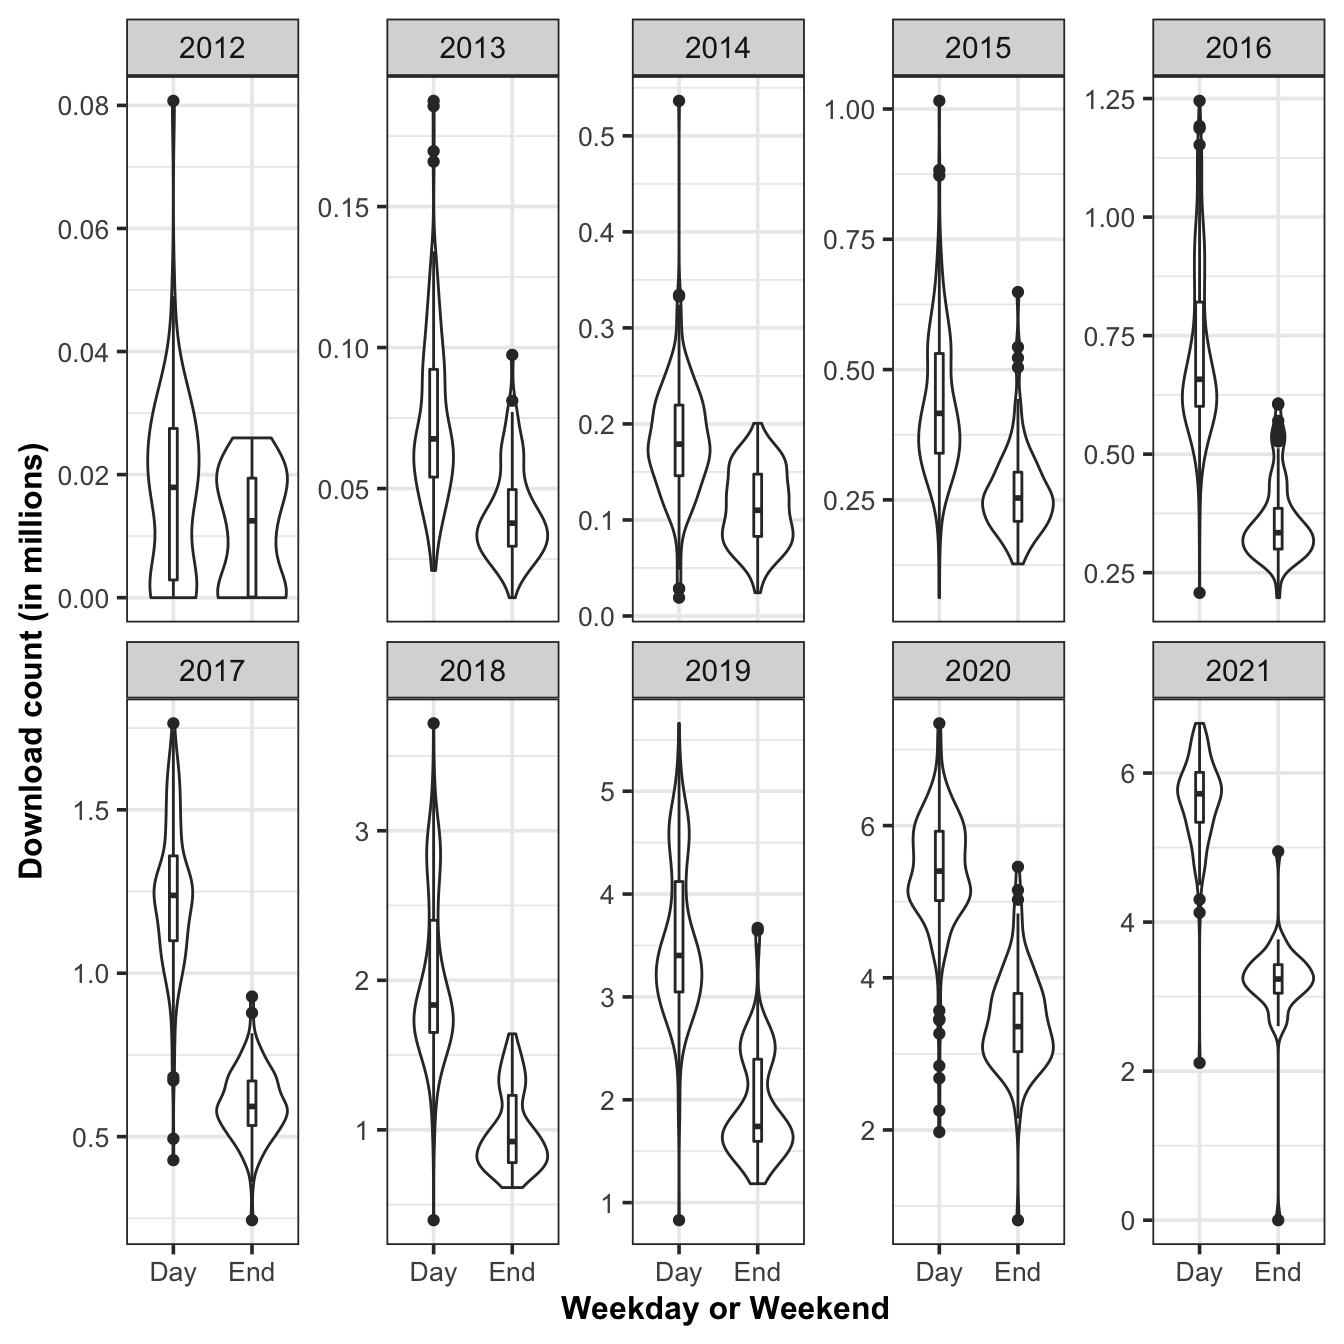
\includegraphics{figures/weekend-vs-weekday-1} 

}

\caption{The violin plot for downloads of all of R-packages on CRAN, between weekday and weekends.}\label{fig:weekend-vs-weekday}
\end{figure}

\begin{discovery}
\textbf{Finding 4}: Top 10\% downloaded R-packages share nearly 90\%
cumulative download counts of the whole.
\end{discovery}

From the previous analysis, we could see that the cumulative download counts of R-packages show an increasing trend. It would be perfect equality if every R-package had the same download count : the last 20\% downloaded R-packages would gain 20\% of the total download count or the top 60\% downloaded R-packages would get 60\% of the total download count. But knowing from experience, we know that is hardly possible. So, here, we introduced Lorenz curve\citep{lorenz} to show the respective numbers of R-packages within different download levels (groups defined by quantiles of download counts). In this way, we could figure out how many download counts contributed by different downloaded R-packages.

Figure \ref{fig:lorenz-all} shows cumulative download counts against each downloaded group. It can be seen that most of the download counts come from the top 10\% downloaded R-packages. At the same time, we could also observe that the Gini value is close to 1, which indicates that the download volumes across groups are quite unbalanced. In fact, the download volume of the top 10\% group is extremely distinguished from that of the following groups. It's not hard to understand that this group should contain some R-packages with high popularity and large quantities of users.



\begin{figure}

{\centering 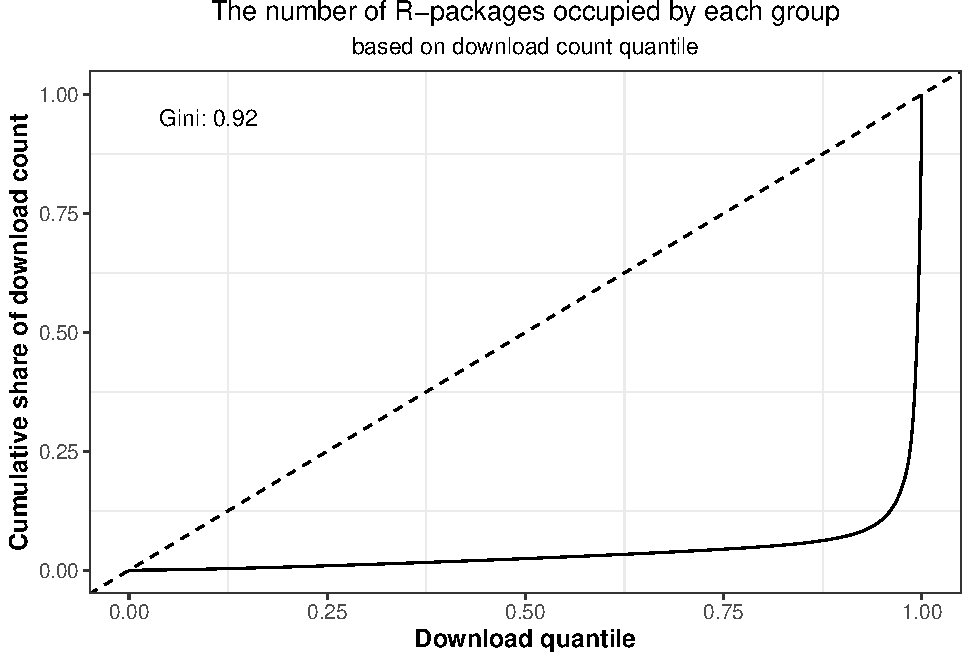
\includegraphics{figures/lorenz-all-1} 

}

\caption{Percentiles of the download counts against cumulative download counts for R-packages at or below that percentile.}\label{fig:lorenz-all}
\end{figure}

For example, if we extracted the first 10 packages of this group in Table \ref{tab:top10}, we could find that there are many quite famous and frequently-used R-packages, such as \texttt{rlang} and \texttt{dplyr}.

\textbackslash begin\{table\}

\textbackslash caption\{\label{tab:top10}First 10 R-packages of top 10\% downloaded group\}
\centering

\begin{tabular}[t]{l|r}
\hline
package & total\\
\hline
rlang & 15572507\\
\hline
vctrs & 13544857\\
\hline
dplyr & 12739206\\
\hline
ggplot2 & 12670952\\
\hline
jsonlite & 12627542\\
\hline
lifecycle & 11124212\\
\hline
tibble & 10935860\\
\hline
magrittr & 10312021\\
\hline
pillar & 9566463\\
\hline
glue & 9534999\\
\hline
\end{tabular}

\textbackslash end\{table\}

\hypertarget{daily-downloads-of-r}{%
\section{Daily downloads of R}\label{daily-downloads-of-r}}

In this section, we studied the daily downloads of R language itself from 2012-10-01 to 2021-06-12. The data was obtained from the \texttt{cranlogs} package \citep{cranlogs} as well.

\begin{discovery}
\textbf{Finding 1}: There is an upward trend in the number of downloads,
also with an increasing variance.
\end{discovery}

Figure \ref{fig:R-download-trend} shows the download trend of R on CRAN over the period of time, from 2012-10-01 to 2021-06-12. An upward trend shows, with an increasing variance in download counts, which is resulted from the growth of R users. As for significant spikes, they are probably quite similar to the situation of R-packages, which is due to repeated downloads, weekly calendar effect or server test issue.



\begin{figure}

{\centering 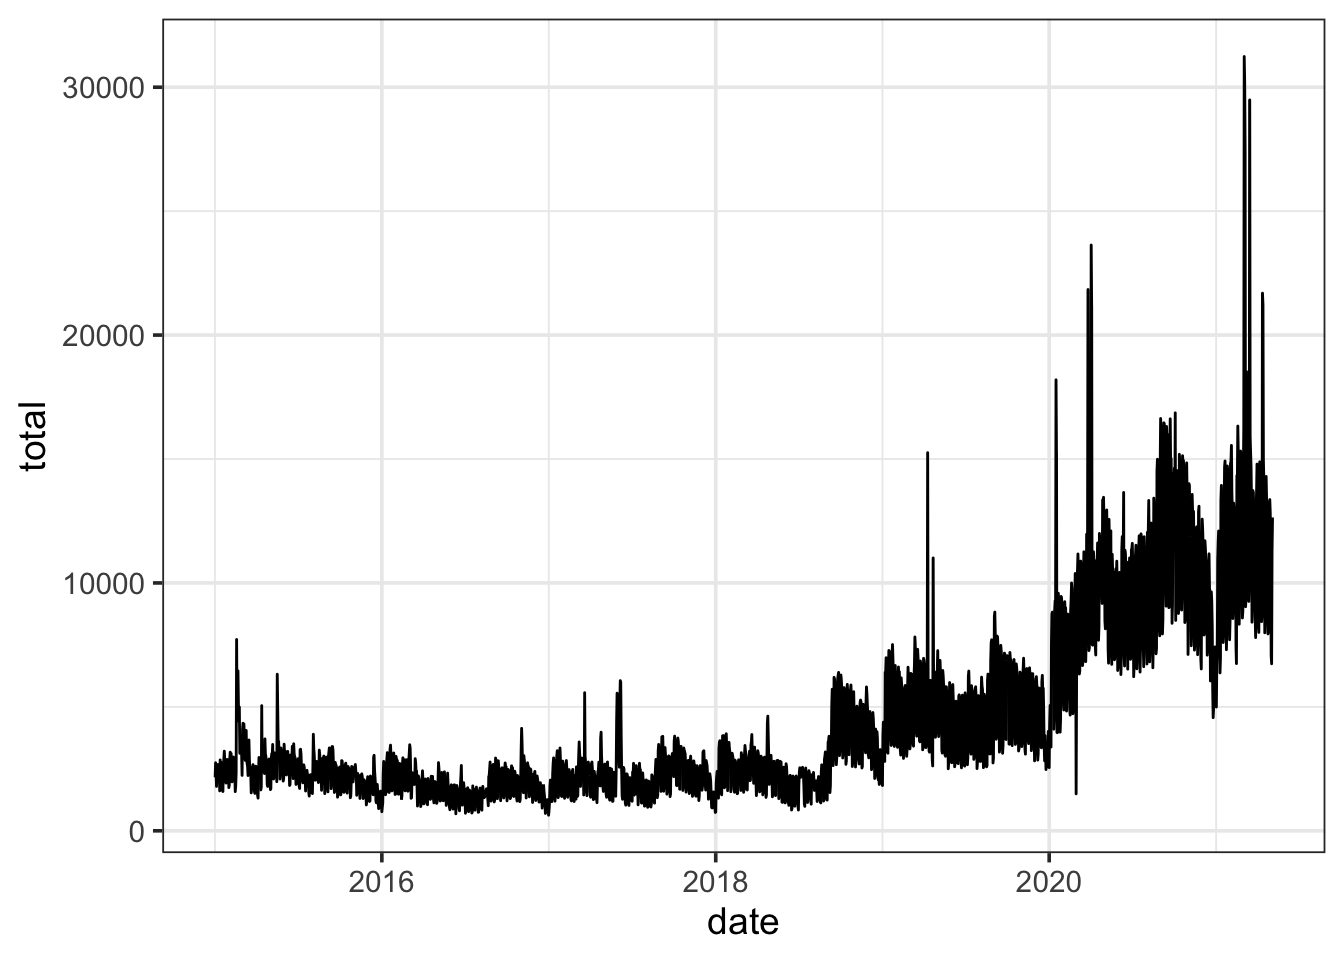
\includegraphics{figures/R-download-trend-1} 

}

\caption{The download trend of R on CRAN, from 2012-10-01 to 2021-06-12.}\label{fig:R-download-trend}
\end{figure}

\begin{discovery}
\textbf{Finding 2}: The most used operation system for R users turns out
to be Windows OS.
\end{discovery}

Figure \ref{fig:R-download-trend-os} shows the comparison of operation systems for R users. The number of Windows-user ranks first, followed by MacOS and SRC. Microsoft has traditionally dominated the desktop and laptop market. And Microsoft officially claims there are 400 million active users of Windows 10 itself, while Apple revealed that there are only around 100 million active Mac users, up to now.\citep{warren2017}



\begin{figure}

{\centering 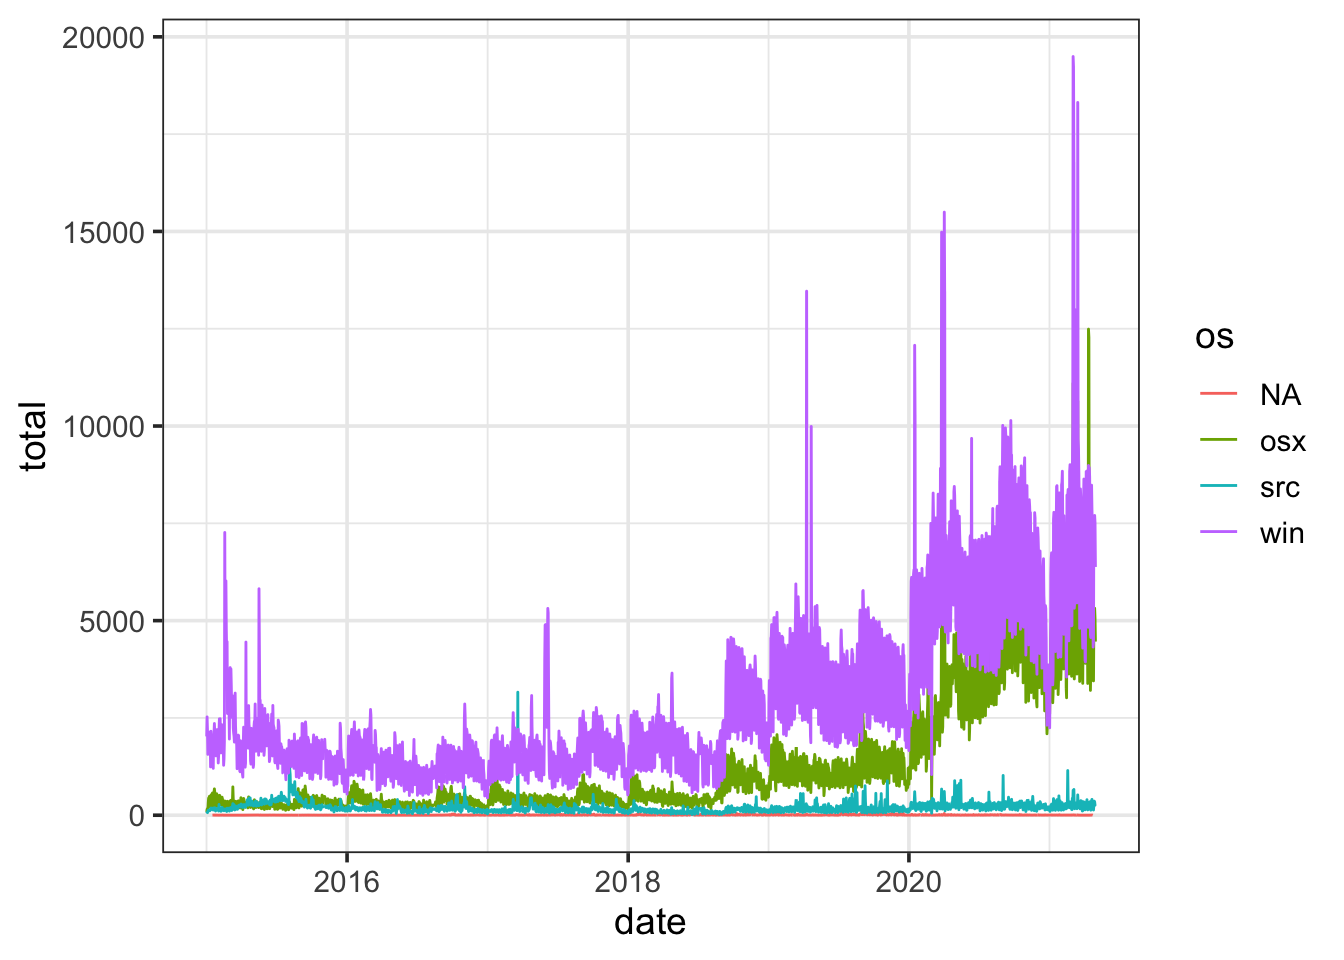
\includegraphics{figures/R-download-trend-os-1} 

}

\caption{The comparison of operation system (OS) for R users, from 2012-10-01 to 2021-06-12.}\label{fig:R-download-trend-os}
\end{figure}

\begin{discovery}
\textbf{Finding 3}: The most popular version of R is 3.2.1
\end{discovery}

Table \ref{tab:R-download-trend-version} shows the first 10 numbers of downloads for different versions of R. The most downloaded one is 3.2.1 with 4526 times, followed by 3.3.3 with 4305 times and 3.1.2 with 3958 times. Most users are likely to install the latest version of R to get the newest update information.

\begin{table}

\caption{\label{tab:R-download-trend-version}The numbers of downloads for different versions of R}
\centering
\begin{tabular}[t]{l|r}
\hline
R\_version & count\\
\hline
3.2.1 & 4526\\
\hline
3.3.3 & 4305\\
\hline
3.1.2 & 3958\\
\hline
3.2.2 & 3781\\
\hline
3.4.0 & 3585\\
\hline
3.1.1 & 3458\\
\hline
3.5.1 & 3450\\
\hline
3.4.3 & 3409\\
\hline
3.4.1 & 3398\\
\hline
3.3.0 & 3362\\
\hline
\end{tabular}
\end{table}

In conclusion, the daily download trends of R are quite similar to those of R-packages, and they are both significantly correlated to weekly calendar as well as unusual downloads from CRAN mirrors. In general, they both tend to increase with the growing of R users.

\hypertarget{daily-top-15-downloaded-r-packages}{%
\section{Daily top 15 downloaded R-packages}\label{daily-top-15-downloaded-r-packages}}

In this section, we studied the top 15 downloaded R-packages from \texttt{2013-04-01} to \texttt{2021-04-01}, to see how user preferences have been changing. The data were obtained from CRAN website {[}\url{http://cran.rstudio.com/web/packages/packages.rds}{]}.

We are supposed to know that some R-packages are hold by Rstudio, some are developed by core personnel or personnel closely related to R, and some are created by prolific developers\citep{revolutions}. And there are also parts of R-packages that are dependency packages of others, which means the increasing downloads of their ``father'' packages would also promote the downloads of them. For example, R-package \texttt{fable} is dependency package within R-package \texttt{fpp3}. When users install \texttt{fpp3}, \texttt{fable} would also be installed at the same time. Naturally, the numbers of downloads for those packages can probably be higher. On the one hand, the R-packages developed by those experienced developers may be more mature and completed. On the other hand, users are more inclined to use packages produced by famous authors, which can be regarded as a kind of ``good use'' guarantee.

However, the existence of those packages can cause the results of user preferences biased. Therefore, we decided to explore the R-packages constructed by non-special creators, and screened out four types of R-packages, namely:

\begin{itemize}
\tightlist
\item
  R-packages maintained by R studio
\item
  R-packages created by authors from R core group
\item
  R-packages created by authors from R secondary group
\item
  R-packages created by R related authors
\item
  R-packages created by top 20 prolific maintainers (This is resourced at \citet{revolutions})
\end{itemize}

After that, we generated a lorenz curve here again in Figure \ref{fig:lorenz-filter}, it can be observed that the distribution of R-packages in each download group is more equal now and the Gini value decreases as well, for the `extreme effect' brought by highly-downloaded packages has disappeared. Thus, the user preferences could be shown more clearly. However, after filtering, the number of remaining R-packages is only 58, which is a too small-sized sample to conduct representative conclusions, we would still focus on all of R-packages on CRAN in later analysis.



\begin{figure}

{\centering 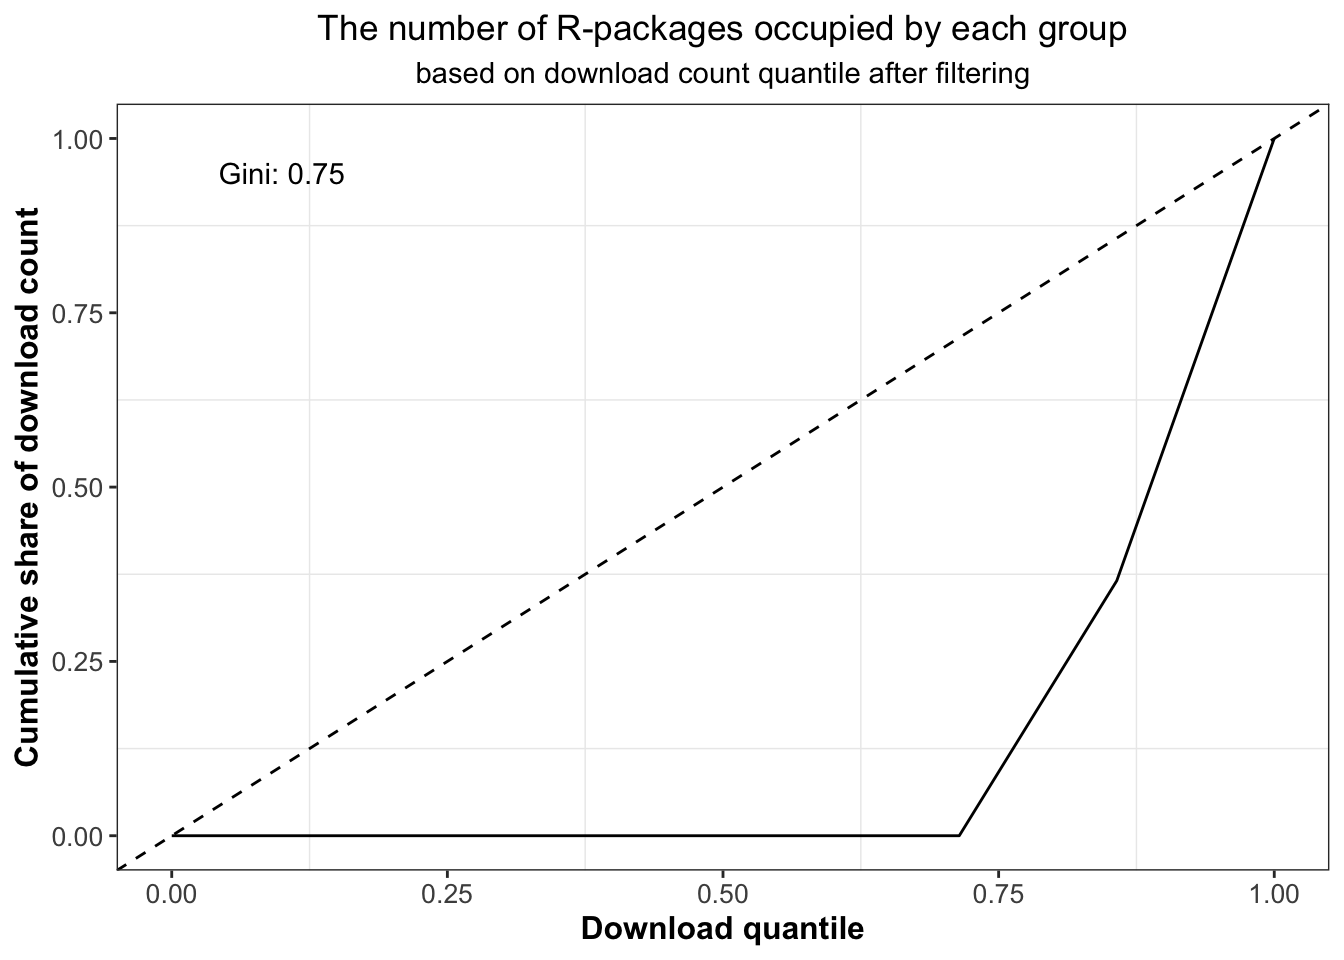
\includegraphics{figures/lorenz-filter-1} 

}

\caption{Percentiles of the download counts against cumulative download counts of R-packages after filtering four types of popular and highly-downloaded packages.}\label{fig:lorenz-filter}
\end{figure}

\begin{discovery}
\textbf{Finding 1}: The topic of newly added R-packages come from quite
different application areas, each year.
\end{discovery}

Table \ref{tab:changed-top15pkg} shows the R-packages that newly come up to the top 15 list each year, from which we can know how the user preferences have changed year by year, compared with the previous year. To be more specific :

\begin{itemize}
\tightlist
\item
  For 2014, \texttt{ncdf} ranks first, which is used to provide an interface to netCDF format data.
\item
  For 2015, the first downloaded R-package is \texttt{XLConnectJars}, related to JAVA dependency.
\item
  For 2016, the first downloaded R-package is \texttt{reports}, for standardising the output of R.
\item
  For 2017, \texttt{lava.tobit} aims to help with estimation and simulation of latent variable models.
\item
  For 2018, the first-ranking \texttt{ReportsRs} is for creating Microsoft Word and Powerpoint documents.
\item
  For 2019, \texttt{CALIBERrfimpute} is used to impute missing values in analysis datasets using full conditional specifications.
\item
  For 2020, \texttt{SparkR} is similar to \texttt{dplyr} but for large datasets.
\item
  For 2021, \texttt{heatmap.plus} is an extension of \texttt{heatmap()} function.
\end{itemize}

\begin{table}

\caption{\label{tab:changed-top15pkg}Changed top 15 downloaded R-packages from 2013 to 2019}
\centering
\begin{tabular}[t]{l|l|l|l|l|l|l|l}
\hline
package14\_13 & package15\_14 & package16\_15 & package17\_16 & package18\_17 & package19\_18 & package20\_19 & package21\_20\\
\hline
ncdf & XLConnectJars & reports & lava.tobit & ReporteRs & freetypeharfbuzz & ENmisc & heatmap.plus\\
\hline
playwith & KoNLP & moonsun & rggobi & OceanView & replyr & CoxBoost & lazyrmd\\
\hline
DMwR & doRedis & rPython & alr3 & ReporteRsjars & zipcode & gWidgetstcltk & packagedocs\\
\hline
latticist & ElemStatLearn & rmongodb & tnam & gWidgetsRGtk2 & rmosek & citr & robcp\\
\hline
bstats & testthatsomemore & maxent & SweaveListingUtils & d3heatmap & msgpack & EMMIXskew & skedastic\\
\hline
geoRglm & adehabitat & SDMTools & ElemStatLearn & - & - & RcmdrPlugin.mosaic & nws\\
\hline
reports & wmtsa & MSBVAR & zipcode & - & - & RcmdrPlugin.qual & optimbase\\
\hline
- & mixOmics & d3heatmap & - & - & - & OceanView & SpaDES\\
\hline
- & DatABEL & ReporteRs & - & - & - & - & SpaDES.core\\
\hline
- & - & - & - & - & - & - & bomrang\\
\hline
- & - & - & - & - & - & - & snipEM\\
\hline
- & - & - & - & - & - & - & SpaDES.addins\\
\hline
- & - & - & - & - & - & - & swissdd\\
\hline
\end{tabular}
\end{table}

\begin{discovery}
\textbf{Finding 2}: The topic of R-packages changes least during 2017
and 2019. The most popular application filed is on JAVA dependency.
\end{discovery}

Table \ref{tab:unchanged-top15pkg} shows the R-packages that remain unchanged each year, compared to the previous year, from which we can know which packages are relatively stable in popularity.

To be more specific, packages like \texttt{XLConnectJars}, \texttt{DMwR}, \texttt{KoNLP}, and \texttt{gWidgets} are relatively popular through years from 2014 to 2021. They are used for providing JAVA dependency, data mining, linguistic research and providing API for building toolkit-independent, interactive GUIs.

\begin{table}

\caption{\label{tab:unchanged-top15pkg}Unchanged top 15 downloaded R-packages from 2013 to 2019}
\centering
\begin{tabular}[t]{l|l|l|l|l|l|l|l}
\hline
package14\_13 & package15\_14 & package16\_15 & package17\_16 & package18\_17 & package19\_18 & package20\_19 & package21\_20\\
\hline
Defaults & ncdf & XLConnectJars & XLConnectJars & XLConnectJars & XLConnectJars & freetypeharfbuzz & freetypeharfbuzz\\
\hline
RSQLite.extfuns & epicalc & KoNLP & KoNLP & DMwR & KoNLP & DMwR & OceanView\\
\hline
gWidgetsRGtk2 & gWidgets & DMwR & DMwR & KoNLP & DMwR & gWidgets & -\\
\hline
gWidgets & gWidgetsRGtk2 & gWidgets & reports & SDMTools & SDMTools & d3heatmap & -\\
\hline
alr3 & DMwR & mixOmics & maxent & reports & gWidgets & alr3 & -\\
\hline
epicalc & alr3 & gWidgetsRGtk2 & SDMTools & mixOmics & ElemStatLearn & gWidgetsRGtk2 & -\\
\hline
rggobi & - & - & mixOmics & ElemStatLearn & reports & reports & -\\
\hline
its & - & - & gWidgets & alr3 & gWidgetsRGtk2 & - & -\\
\hline
- & - & - & - & maxent & d3heatmap & - & -\\
\hline
- & - & - & - & gWidgets & alr3 & - & -\\
\hline
\end{tabular}
\end{table}

Next, we changed the object to trending R-packages. Trending R-packages are ones downloaded at least 1000 times last week, which have increased significantly compared to the average weekly downloads in the previous 24 weeks\citep{r-hub}. That is to say, they are packages with significantly high download volume in a recent short time. Through their topics, we can know what application areas of R-packages that people are concerned about recently.

\begin{discovery}
\textbf{Finding 3}: The most popular topic of trending R-packages.
\end{discovery}

Table \ref{tab:trending-count} shows the top 10 downloaded topics for trending R-packages. The most popular topic is Multivariate, followed by Cluster and Phylogenetics. This is easy to understand : the numbers of users from different fields are different, so the downloads of R-packages in different topics also varies. It seems that Multivariate is quite heated recently.

\begin{table}

\caption{\label{tab:trending-count}Ranking topics of trending R-packages}
\centering
\begin{tabular}[t]{l|r}
\hline
topic & download times\\
\hline
Multivariate & 4\\
\hline
Cluster & 3\\
\hline
Phylogenetics & 3\\
\hline
TimeSeries & 3\\
\hline
WebTechnologies & 3\\
\hline
Distributions & 2\\
\hline
ExperimentalDesign & 2\\
\hline
SocialSciences & 2\\
\hline
ClinicalTrials & 1\\
\hline
Finance & 1\\
\hline
\end{tabular}
\end{table}

Apart from the topics of R-packages, what other factors can probably be linked to download volumes? With this question in mind, we then explored the relationship between the total number of download counts for all of CRAN R-packages and the earliest release date in the past year. We also studied the relationship between the total download volume and the number of updates, the number of commits on master (main) branch in GitHub repositories, the lengths and the alphabetical order of names, over the most recent 6 month period, in the following sections.

\hypertarget{compare-last-years-downloads-with-the-initial-release-date}{%
\section{Compare last year's downloads with the initial release date}\label{compare-last-years-downloads-with-the-initial-release-date}}

\begin{discovery}
\textbf{Finding}: R-packages that are initially released earlier on CRAN
tend to have higher download counts in the past year. That is perhaps
because, in earlier times, there were fewer R-packages in the same
category, then users had `no choice' but to use them. Due to that, those
R-packages would accumulate user base, which makes it more possible to
attract new users.
\end{discovery}

In our common cognition, it may be assumed that the earlier an R-package is released, the more people can get to know it, and thus the more downloads it can have. However, R-packages related to different topics cannot be directly compared, because download counts of R-packages in one topic can be higher than that in another. Therefore, in order to test this conjecture as clearly as possible, we selected three domain R-packages through CRAN task view\citep{crantaskviews}, calculated their respective downloads in the previous one year, and extracted their earliest release dates for comparison. Those three topics are :

\begin{itemize}
\tightlist
\item
  R-packages for Time Series Analysis
\end{itemize}

The first topic is Time Series Analysis. Time Series Analysis is a statistical technique that deals with time series data, or trend analysis. Time series data means that data is in a series of particular time periods or intervals\citep{timeseries}.

\begin{itemize}
\tightlist
\item
  Bayesian R-packages for general model fitting
\end{itemize}

The second topic is Bayesian Inference. Bayesian statistics is a mathematical procedure that applies probabilities to statistical problems. It provides people the tools to update their beliefs in the evidence of new data\citep{bayesian}.

\begin{itemize}
\tightlist
\item
  Econometrics R-packages
\end{itemize}

The last topic is related to econometrics. Econometrics is the use of statistical methods using quantitative data to develop theories or test existing hypotheses in economics or finance, which relies on techniques such as regression models and null hypothesis testing\citep{econometrics}.

Figure \ref{fig:release-downloads} displays the scatterplot of the past year's download counts and the earliest release dates, for \texttt{Time\ Series\ Analysis}, \texttt{Econometrics} and \texttt{Bayesian} R-packages. It can be seen that, generally, as the earliest release dates get later and later, the numbers of download logs become lower and lower. For \texttt{Time\ Series\ Analysis} R-packages, they are mainly released between 2012 and 2019. For \texttt{Bayesian} R-packages, most of the R-packages are born from 2007 to 2012. And most \texttt{Econometrics} are centered between 2013 and 2016.



\begin{figure}

{\centering 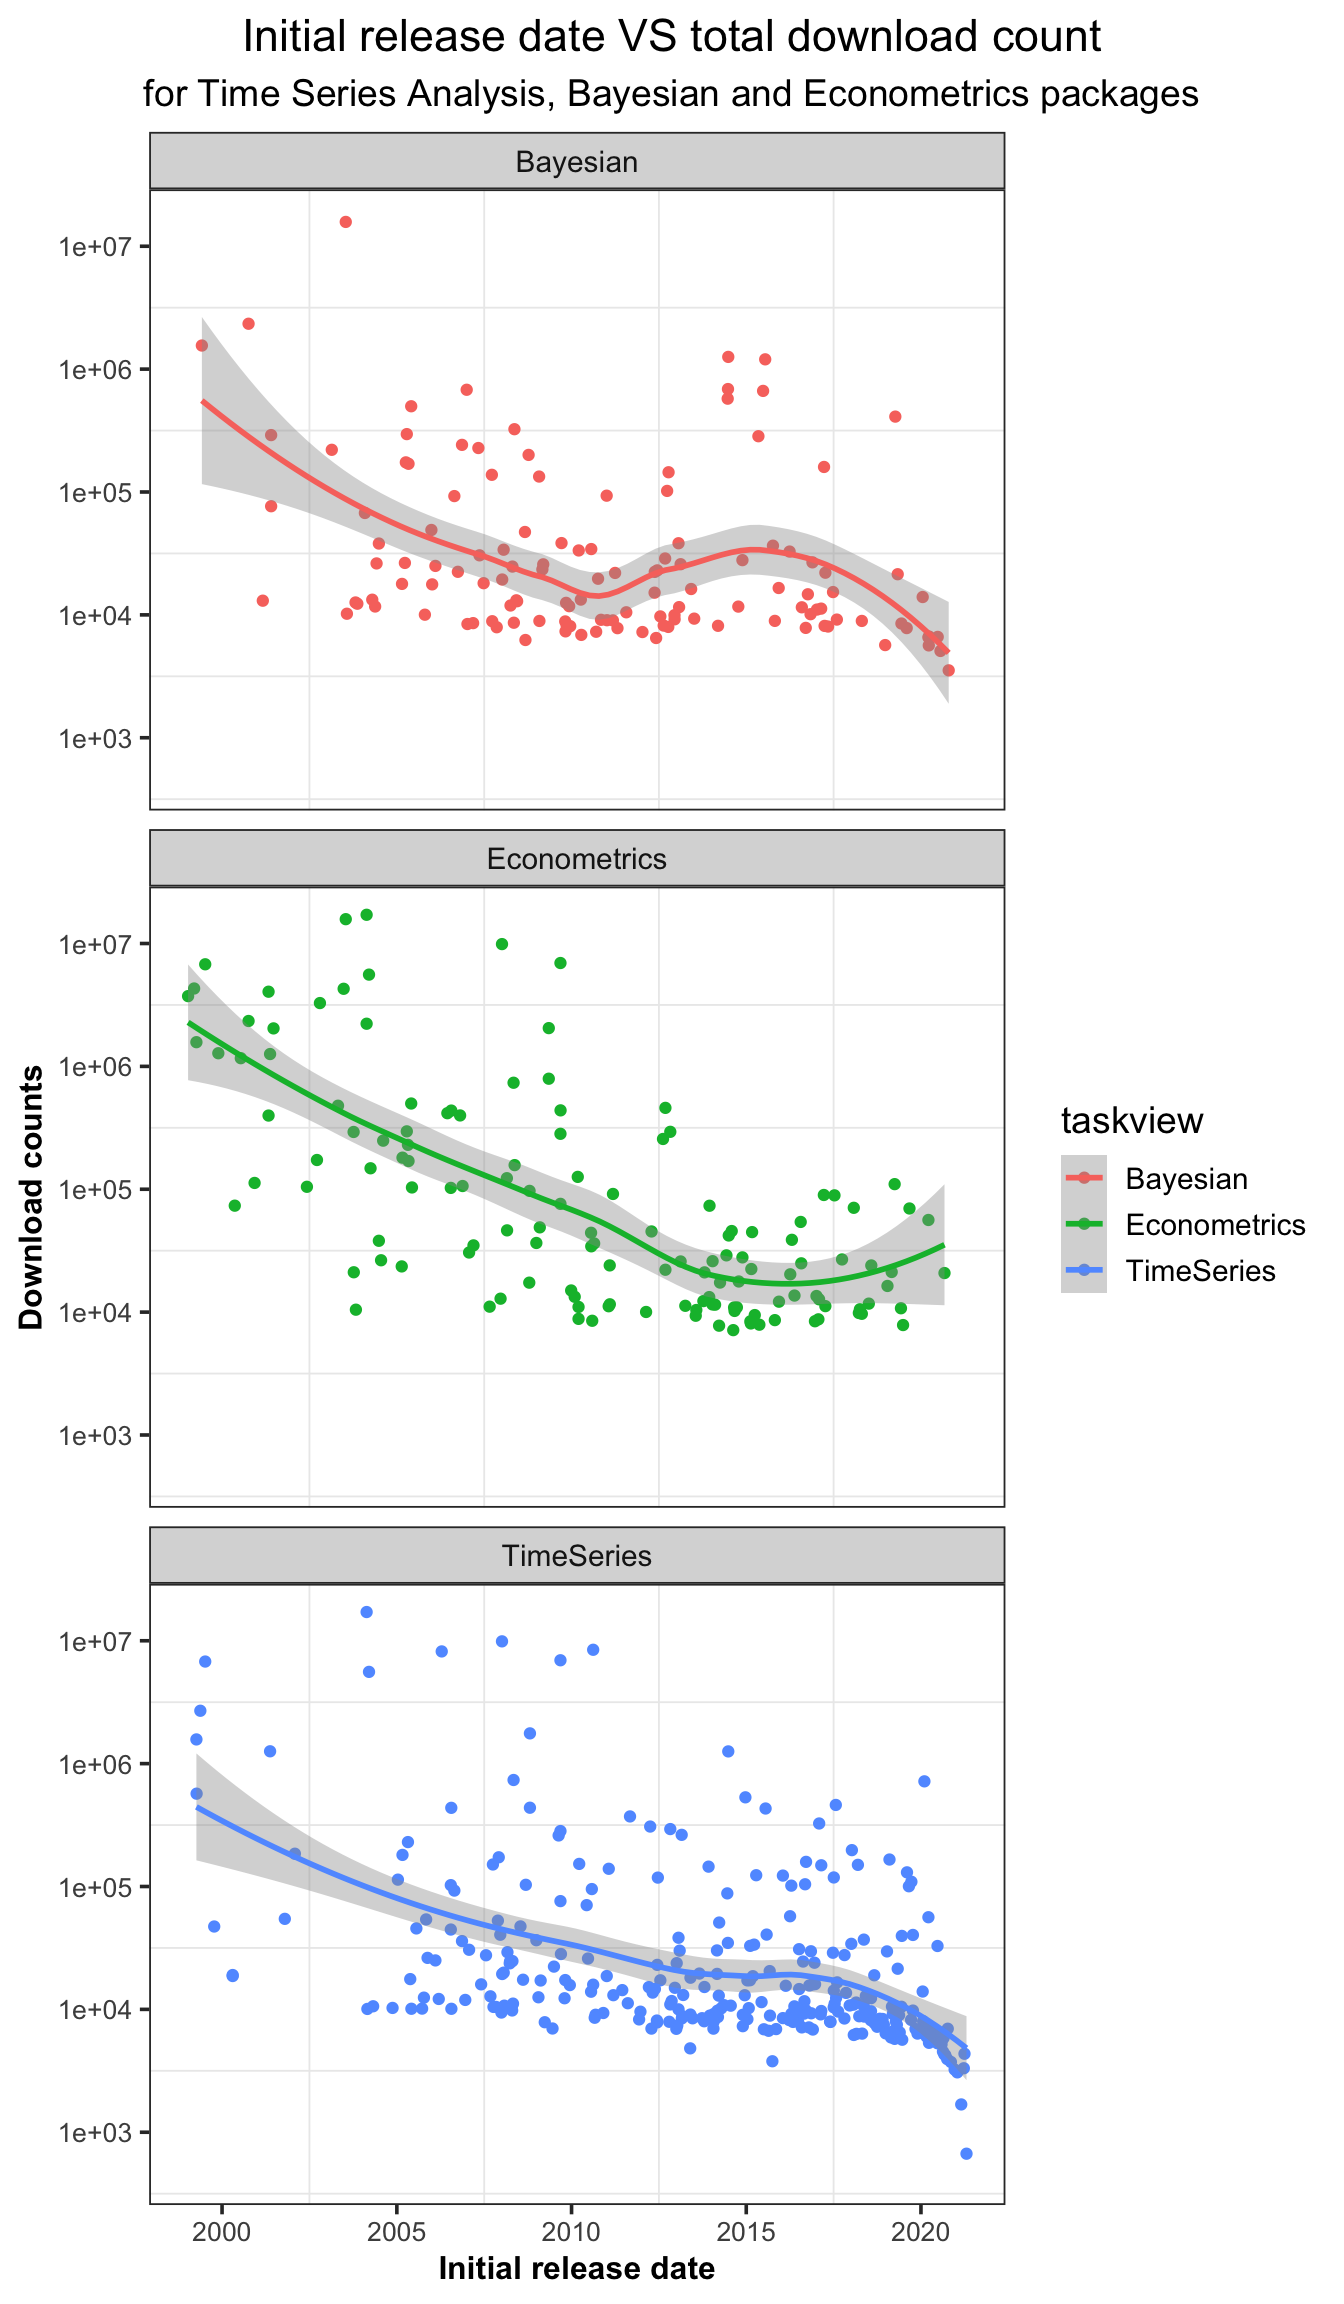
\includegraphics{figures/release-downloads-1} 

}

\caption{The download counts decrease with the initial release dates.}\label{fig:release-downloads}
\end{figure}

In conclusion, it is not surprising to find that the earlier the R-package is released, the more downloads it could have, which is reflected in all of three topics above. That is probably because the R-packages released earlier can be better-known. When they are released early, there may be a relatively small number of R-packages in the same topic, under non-serious competition. As a result, the R-packages coming later can easily be covered up, since people may generally tend to use well-known, mature and habitual packages.

That is to say, earlier R-packages are more conducive to the cultivation of user habits. After all, habits are influenced by the length of time. For example, if the teacher is a senior user of an R-package, they may recommend that R-package to their students when teaching, especially when they obtain a satisfying user experience.

\hypertarget{compare-moving-average-trends-for-fable-and-forecast}{%
\section{Compare moving average trends for fable and forecast}\label{compare-moving-average-trends-for-fable-and-forecast}}

\begin{discovery}
\textbf{Finding}: R-package `forecast' has a more stable download trend
comparing to `fable'. When `fable' gets updated, its downloads peaked,
while `forecast' suffers a dropping, on the contrast.
\end{discovery}

As stated in the previous section, the earlier an R-package is released, the easier it can be to get a relatively higher total downloads. But that doesn't mean a better growth will exist. Due to that, in this section, we compared package \texttt{fable} and \texttt{forecast}. They are two closely related R-packages, for \texttt{fable} is the later released tidy version of \texttt{forecast}. And in this way, we can approximately fix all of factors, except the initial release date, so that we can compare the growth and changes of those two more clearly.

Figure \ref{fig:daily-fbl} and Figure \ref{fig:daily-fcst} show the daily download counts changing over the most recent 6 month period, with strong weekly seasonality. That means the downloads tend to be higher within week days and thus lower on weekends, which is consistent with trend for all of R-packages that was analyzed before.



\begin{figure}

{\centering 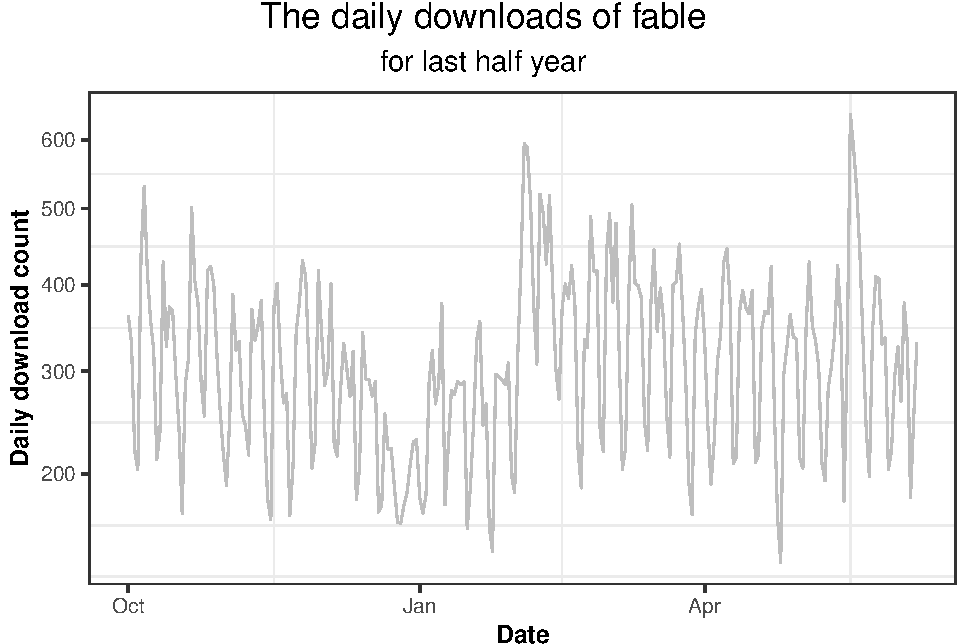
\includegraphics{figures/daily-fbl-1} 

}

\caption{The daily downloads of R-package ``fable''}\label{fig:daily-fbl}
\end{figure}



\begin{figure}

{\centering 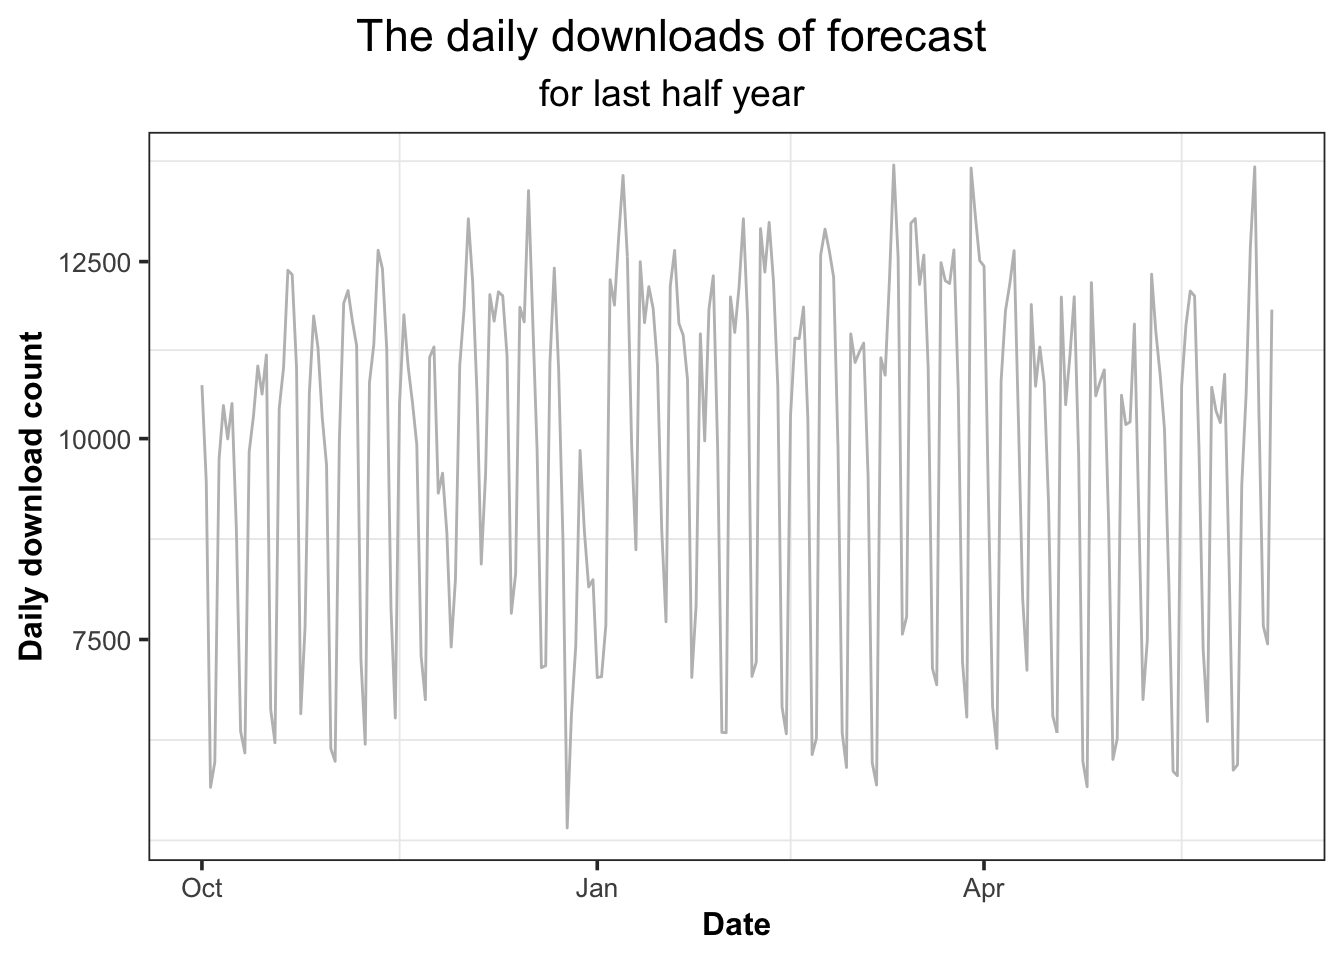
\includegraphics{figures/daily-fcst-1} 

}

\caption{The daily downloads of R-package ``forecast''.}\label{fig:daily-fcst}
\end{figure}

Therefore, in order to estimate the trend-cycle and reduce the weekly seasonality, to see the changes more clearly, the Moving Average (MA) was introduced\citep{movingaverage}.

A moving average of order \textbf{m} can be written as :

\[T_t = \frac1m\ \Sigma_{j = -k}^{k}y_{t+j} \]

where \textbf{m=2k+1}. That is, the estimate of the trend-cycle at time \textbf{t} is obtained by averaging values of the time series within \textbf{k} periods of \textbf{t}.

And here, we considered an equal weighed 7 moving average. It calculates the weighted average for every seven consecutive time series with the following weights : \emph{{[}1/7,1/7,1/7,1/7,1/7,1/7,1/7{]}}.

Figure \ref{fig:ff-ma} shows the moving average (MA) of \texttt{fable} and \texttt{forecast} respectively. They have quite different moving average patterns, when \texttt{forecast}'s download volume is much higher than that of \texttt{fable}, except for the time around New Year's Eve, with a significant drop in \texttt{forecast}. But during that time, a drop also appears in \texttt{fable}, which was probably due to the big New Year holiday. In addition, the purple vertical dashed line in plot of \texttt{fable} marks the update day of it, on 2021-1-29. Soon after that day, \texttt{fable}'s downloads peaked, which was due to the increase brought by update day. At the same time, \texttt{forecast} drops, then only gets a gentle increase.



\begin{figure}

{\centering 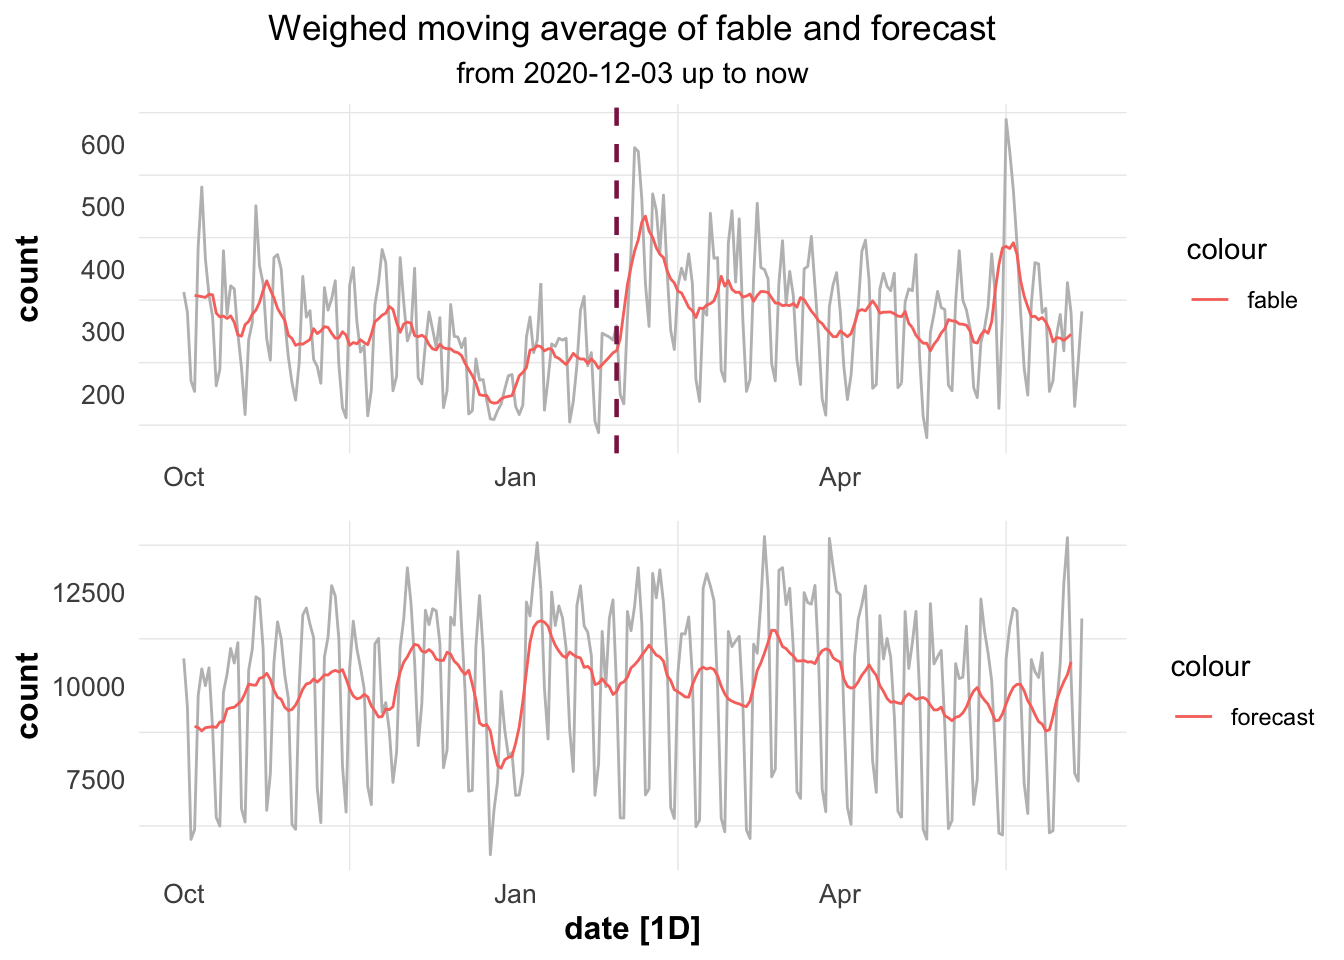
\includegraphics{figures/ff-ma-1} 

}

\caption{The moving averages of R-package ``forecast'' and ``fable''.}\label{fig:ff-ma}
\end{figure}

In conclusion, the download variance of \texttt{forecast} is larger than that of \texttt{fable} while the former looks relatively more stable than the latter, after applying the moving average. It coincides with the conclusion of the previous section : the earlier released R-package tends to obtain more cumulative downloads. In addition, we can also see that the growths of both of two sometimes increase at the same time, while the growth of one can correspond to the decline of the other, sometimes. As for as we concerned, the shared growth may be due to their similarity. Users may download both at the same to compare, like us. And the trade-off may also be due to their similar functions, one can be replaced by the other. Finally, earlier release does not guarantee a faster growth. For example, \texttt{fable} has a more dramatic growth than \texttt{forecast} from 2021-01-21 to 2021-02-06.

\hypertarget{compare-download-counts-with-the-number-of-commits-on-master-branch}{%
\section{Compare download counts with the number of commits on master branch}\label{compare-download-counts-with-the-number-of-commits-on-master-branch}}

In this section, we compared total downloads over the most recent 6 month period, with the number of commits on master branch in Github repositories. For all of CRAN R-packages, there were only 6185 R-packages that have Github repositories, and after cleaning up, only 5769 remained.

\begin{discovery}
\textbf{Finding}: In our initial assumption, more commits on master
branch of Github repositories are likely to bring R-packages more
download counts. On the one hand, the number of commits can indicate
that developers are constantly supplementing and updating their
R-packages, which may lead to more downloads. On the other hand, the
number of commits also can reflect the attention developers attach to
their R-packages, to some extent. Usually, for those who have more
commits, their developers may advertise more or try other ways, to
expand the popularity and improve the download counts.
\end{discovery}

The way we initially planned to apply was extracting the commits through accessing the Github REST API\citep{githubapi}. To achieve that, we first scraped the Github URLs from `description' pages for all of R-packages from CRAN, then cleaned up the multiple URLs and other redundant symbols or characters. The URL is formatted as : \emph{``\url{https://api.github.com/repos/\%7Buser_repo\%7D/commits?per_page=1}''}. For example, the URL for package \texttt{tidyverse} can be like : \emph{``\url{https://api.github.com/repos/tidyverse/tidyverse/commits?per_page=1}''}. Practically, by replacing the \texttt{user\_repo} part that consists of the name of the related repository and the name of the package holder, we could access the contents of URLs through Github API, for all of CRAN R-packages.

Based on that, Table \ref{tab:userrepo-tbl} shows the first 5 R-packages, with their Github URLs and the \texttt{user\_repo} parts.

However, the Github API has a rate limits, allowing for up to 60 requests per hour for unauthenticated requests, which can be extended to 5000 per hour after authentication\citep{githubapi}. But even after getting authentication, our rate limit didn't get promoted. So, we switched to scrape commits with Python spider, by setting random user agent, to avoid the API limit. Since this method is quite time consuming (around 5 hours each time for all available R-packages), we saved the output as a local .txt file and load it later in R studio, to speed up the code execution.

\textbackslash begin\{table\}

\textbackslash caption\{\label{tab:userrepo-tbl}First 5 R-packages with their `user\_repo' element\}
\centering

\begin{tabular}[t]{l|l|l}
\hline
package & URL & user\_repo\\
\hline
abbyyR & http://github.com/soodoku/abbyyR & soodoku/abbyyR\\
\hline
ABCoptim & http://github.com/gvegayon/ABCoptim & gvegayon/ABCoptim\\
\hline
abctools & http://github.com/dennisprangle/abctools & dennisprangle/abctools\\
\hline
abdiv & http://github.com/kylebittinger/abdiv & kylebittinger/abdiv\\
\hline
abess & http://github.com/abess-team/abess & abess-team/abess\\
\hline
\end{tabular}

\textbackslash end\{table\}

Table \ref{tab:commits-tbl} shows the first 5 R-packages of all, along with their total downloads over the most recent 6 month period, and the numbers of commits on master branch in Github repositories.

\begin{table}

\caption{\label{tab:commits-tbl}R-packages with commits on Github and total downloads over the most recent 6 months}
\centering
\begin{tabular}[t]{l|l|r}
\hline
package & commits & total\\
\hline
rlang & 4,427 & 14748569\\
\hline
dplyr & 7150 & 12054840\\
\hline
ggplot2 & 4,756 & 11825489\\
\hline
lifecycle & 206 & 10438007\\
\hline
tibble & 4,286 & 10340887\\
\hline
\end{tabular}
\end{table}

Figure \ref{fig:commits-pattern} shows the scatterplot, along with a smoothing line. In general, more commits can link to more downloads.



\begin{figure}

{\centering 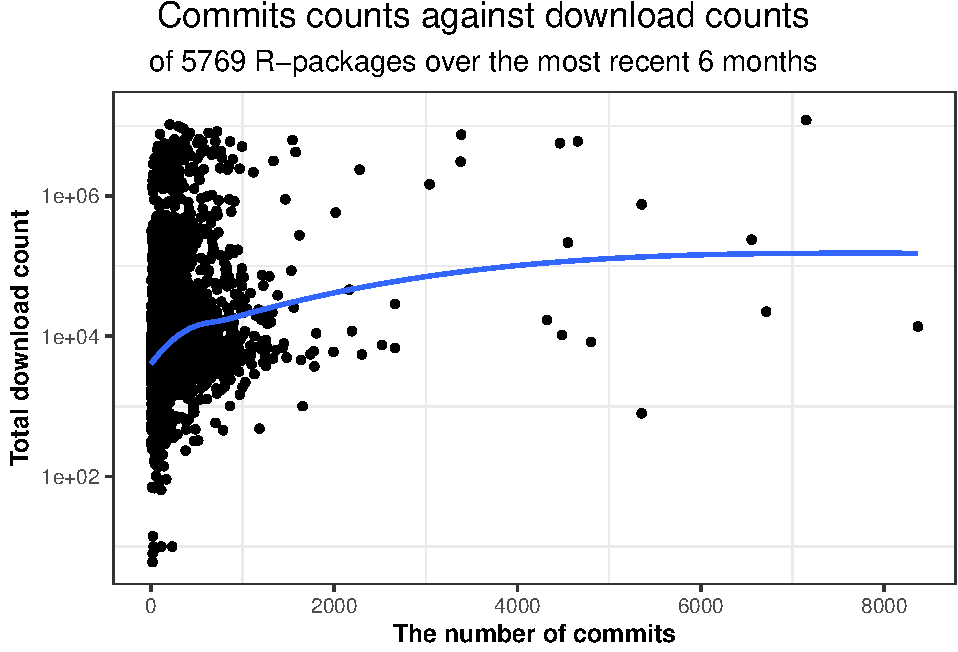
\includegraphics{figures/commits-pattern-1} 

}

\caption{The commits on master branch in Github repositories against the total download counts over the most recent 6 month period.}\label{fig:commits-pattern}
\end{figure}

Another method can be conducted by taking the ultra-low-downloaded R-packages into consideration, whose download counts only rank last 1\% of all. Another purpose for this way is to show our initial idea on scraping commits through Github API with R (as the sample size is less than 60 R-packages, on this condition).

Table \ref{tab:quantileall} shows the last 10 quantiles of download counts, it can be seen that the last 1\% download count is around 375.12. As the download counts of those packages are extremely low, we could assume that many factors can have little effect on their downloads, and the only two differences among them are the numbers of commits on Github master branch and the total download counts.

Based above, we could select those ultra-low-downloaded R-packages and extract commit counts from their Github repositories. In Figure \ref{fig:pkg-low}, it could be observed that when the number of commits increases from 0 to 100, the download counts first increase and then decrease. After that, the download volume keeps rising, with a small jump at the end. We consider that might result from the too small-sized sample, and the observation causing the decline can be an outlier. If expanding the observation horizon, an increase in this curve can be expected. Therefore, it can be concluded that even for those last 1\% downloaded R-packages, the phenomenon - ``the more commits can link to more downloads'' also exists.

\begin{table}

\caption{\label{tab:quantileall}Quantile of total download counts for all of R-packages on CRAN}
\centering
\begin{tabular}[t]{l|r}
\hline
  & download\_count\\
\hline
0\% & 0.00\\
\hline
1\% & 375.12\\
\hline
2\% & 721.56\\
\hline
3\% & 1075.34\\
\hline
4\% & 1340.24\\
\hline
5\% & 1562.70\\
\hline
6\% & 1674.00\\
\hline
7\% & 1804.46\\
\hline
8\% & 1903.24\\
\hline
9\% & 1968.02\\
\hline
\end{tabular}
\end{table}



\begin{figure}

{\centering 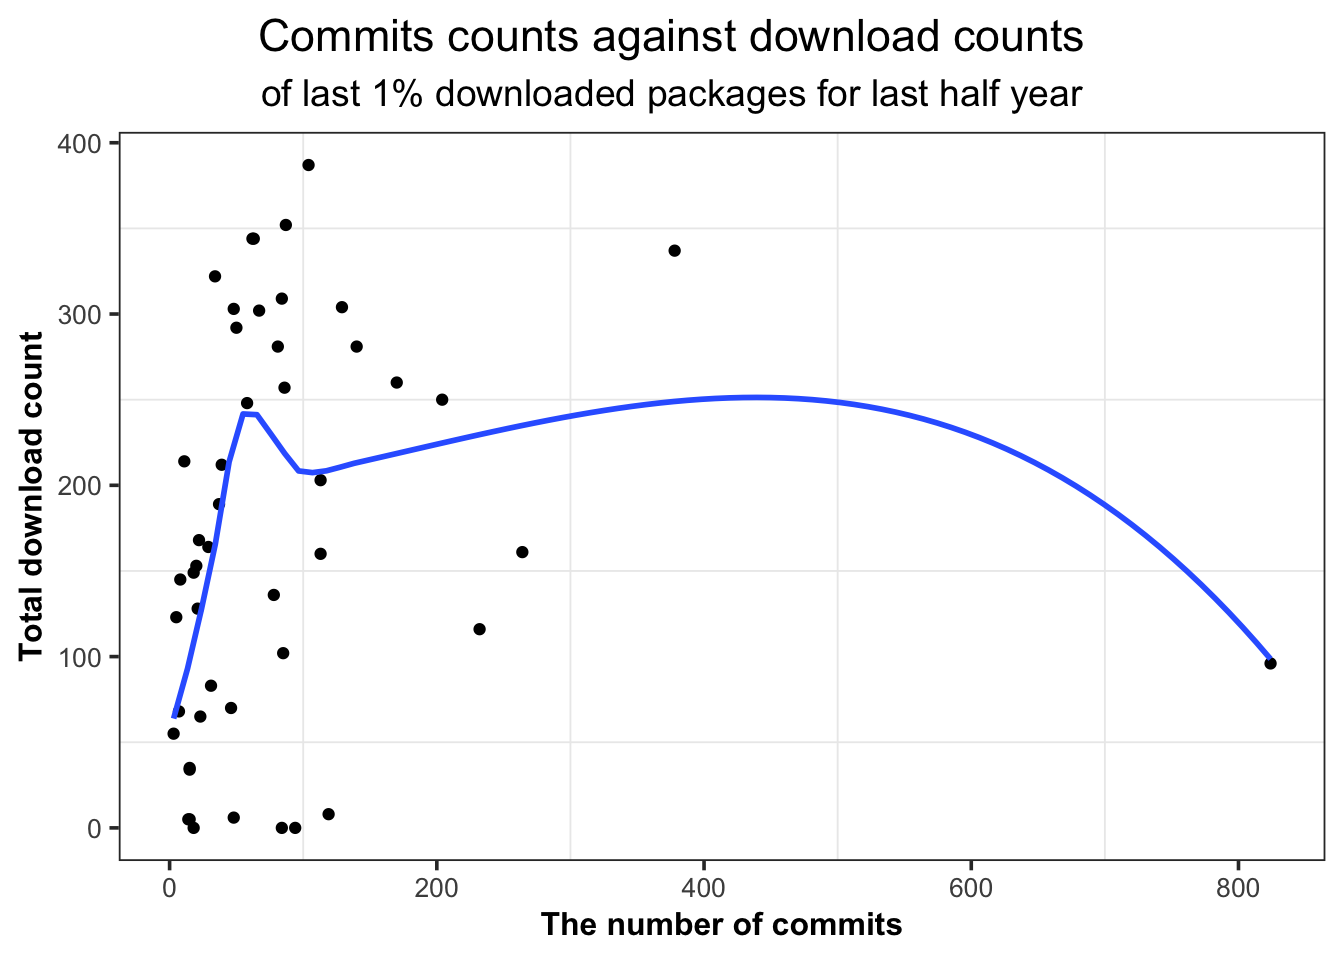
\includegraphics{figures/pkg-low-1} 

}

\caption{The commits on master branch of Github repositories, against the total download counts over the most recent 6 month period, for last 1\% downloaded R-packages on CRAN.}\label{fig:pkg-low}
\end{figure}

\hypertarget{compare-download-counts-with-the-numbers-of-updates}{%
\section{Compare download counts with the numbers of updates}\label{compare-download-counts-with-the-numbers-of-updates}}

In this section, we looked into the relationship between the numbers of updates and total download counts over the most recent 6 month period, for all of CRAN R-packages.

\begin{discovery}
\textbf{Finding 1}: The download counts tend to rise with the numbers of
updates. This is probably because there will be a significant increase
in downloads when packages get updated. During that time, not only old
users often download the latest version, but also it is easier to
attract new users, for the increase of downloads within a short period
of time can bring packages up to the trending list{[}@r-hub{]}.
\end{discovery}

Figure \ref{fig:all-updates} shows that the numbers of downloads increase with the update times. And most R-packages are updated no more than 30 times.



\begin{figure}

{\centering 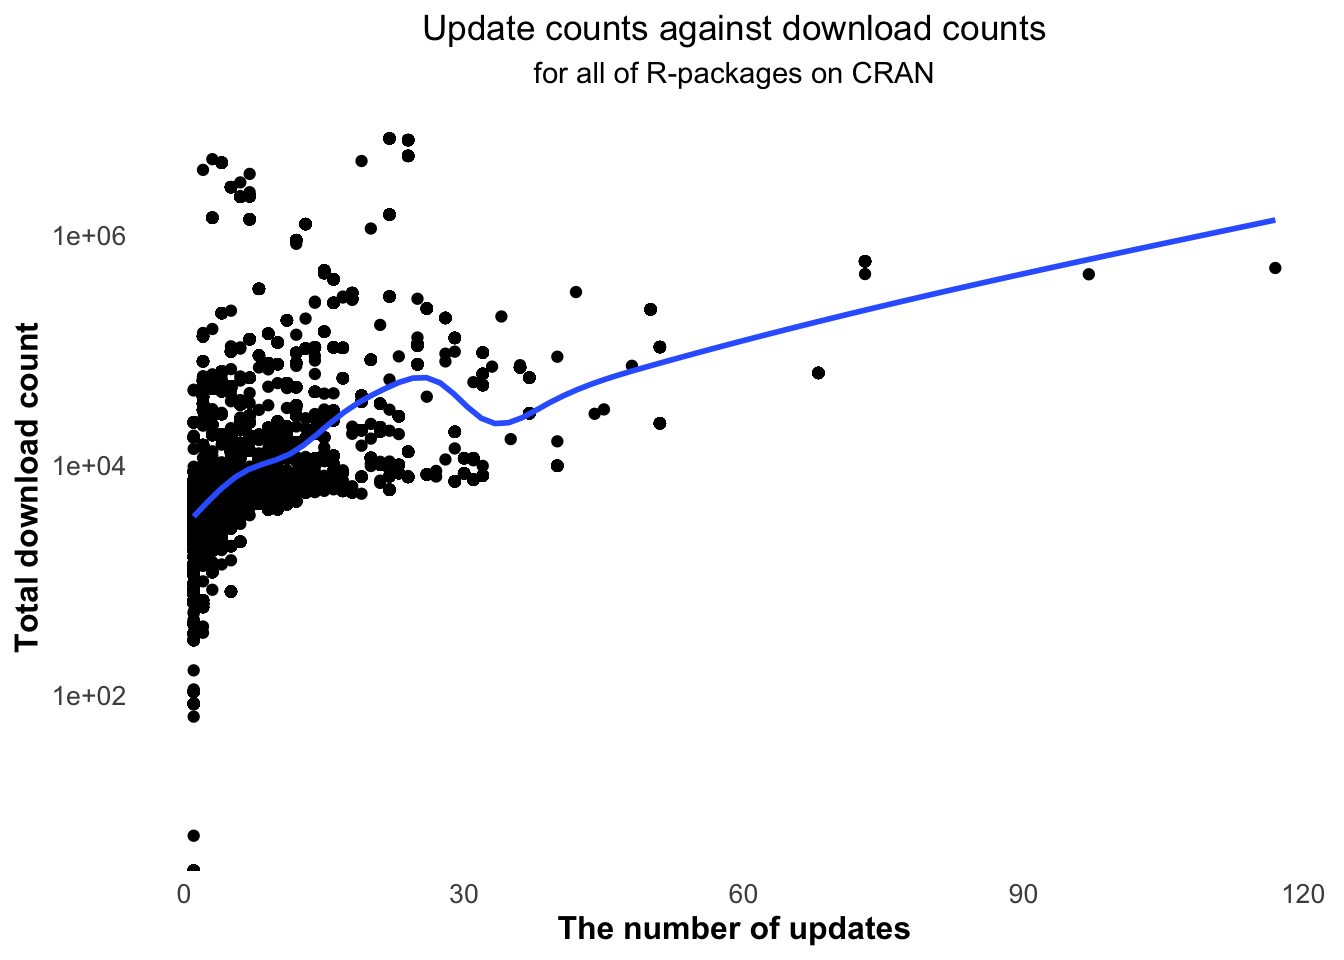
\includegraphics{figures/all-updates-1} 

}

\caption{The download counts increase with the numbers of updates.}\label{fig:all-updates}
\end{figure}

\begin{discovery}
\textbf{Finding 2}: Over half of the CRAN R-packages are not likely to
update very frequently.
\end{discovery}

By checking Table \ref{tab:pct-lowupdates}, we can know that the percentage of R-packages whose updates are less than average is 70.2920266 \%, which means much more than half of the CRAN R-packages do not tend to update very frequently.

\begin{table}

\caption{\label{tab:pct-lowupdates}Percentage of CRAN R-packages whose updates are less than average}
\centering
\begin{tabular}[t]{r|r}
\hline
number of packages with low updates & percentage of packages with low updates\\
\hline
11963 & 70.29203\\
\hline
\end{tabular}
\end{table}

\begin{discovery}
\textbf{Finding 3}: Most CRAN R-packages keep updating with the time,
probably to keep its activity.
\end{discovery}

It can be seen from Figure \ref{fig:latestpublish} that most R-packages' latest publish dates are after 2015, which indicates that many R-packages are likely to update with the time, probably in order to keep their activity.



\begin{figure}

{\centering 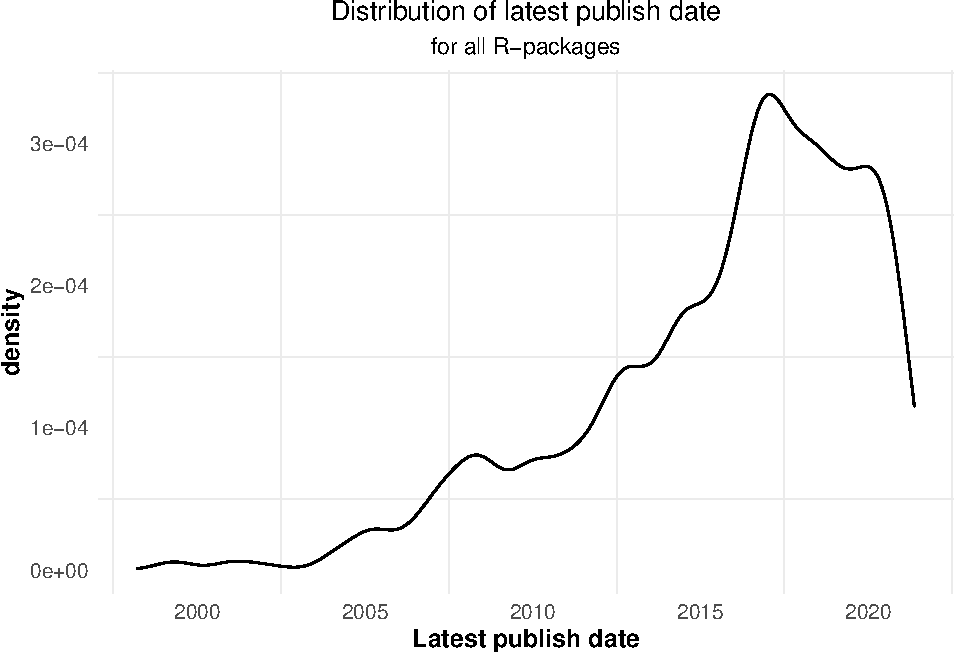
\includegraphics{figures/latestpublish-1} 

}

\caption{The latest update dates of CRAN R-packages are almost the recent dates.}\label{fig:latestpublish}
\end{figure}

\begin{discovery}
\textbf{Finding 4}: Most of the CRAN R-packages are likely to update
with a relatively long time interval.
\end{discovery}

Figure \ref{fig:updates-perday} shows that with the increase of update intervals, the numbers of downloads first increase and then decrease slightly. Most of the time intervals are between 45 and 450 days, which shows that their update frequency is not very high.



\begin{figure}

{\centering 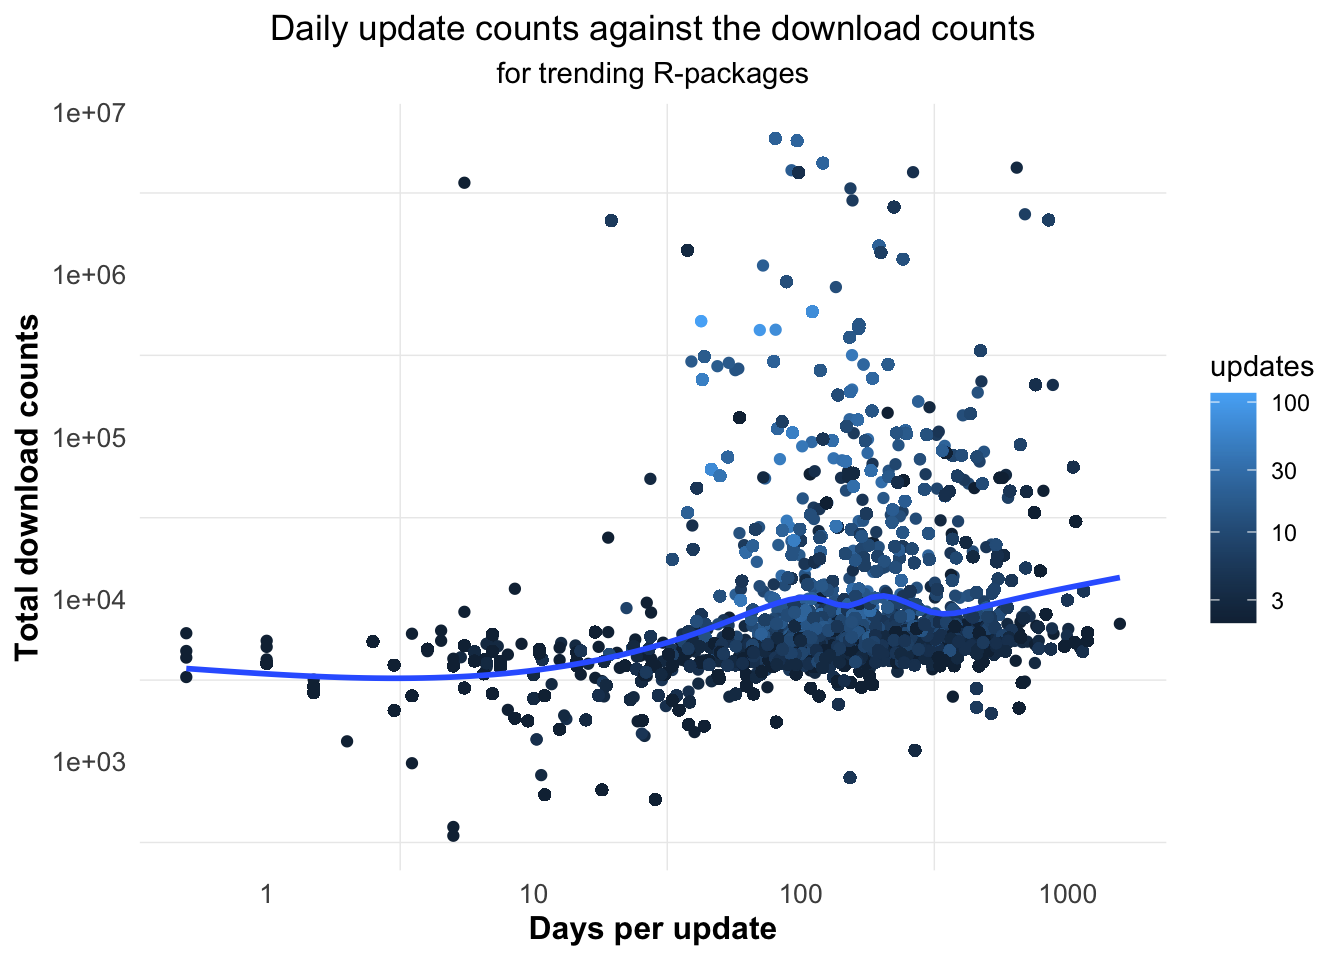
\includegraphics{figures/updates-perday-1} 

}

\caption{Most of the time intervals for updates are between 45 and 450 days.}\label{fig:updates-perday}
\end{figure}

In conclusion, it's not that the more updates R-packages have, the popular they can be. In actual, most of the CRAN R-packages whose updates are lower than average occupy the majority. Therefore, the numbers of updates are probably not that important for R-packages. The really important thing can be keeping updated along the time.

\hypertarget{compare-the-package-name-lengths-with-download-counts}{%
\section{Compare the package name lengths with download counts}\label{compare-the-package-name-lengths-with-download-counts}}

Here, we still focused on all of R-packages on CRAN, and made comparison between their name lengths and total downloads over the most recent 6 month period.

\begin{discovery}
\textbf{Finding 1}: The name lengths of R-packages have no significant
correlation with total downloads, over the most recent 6 month period.
\end{discovery}

We could see from Figure \ref{fig:namelength-plot} that, the influence on download volume resulted from name length is not obvious. But we could still observe that the name lengths of most of R-packages are centered before 10 characters long. The names , with more than 6,000,000 downloads, are between 5 and 9 characters long. The most downloaded one is R-package rlang whose name length is 5.



\begin{figure}

{\centering 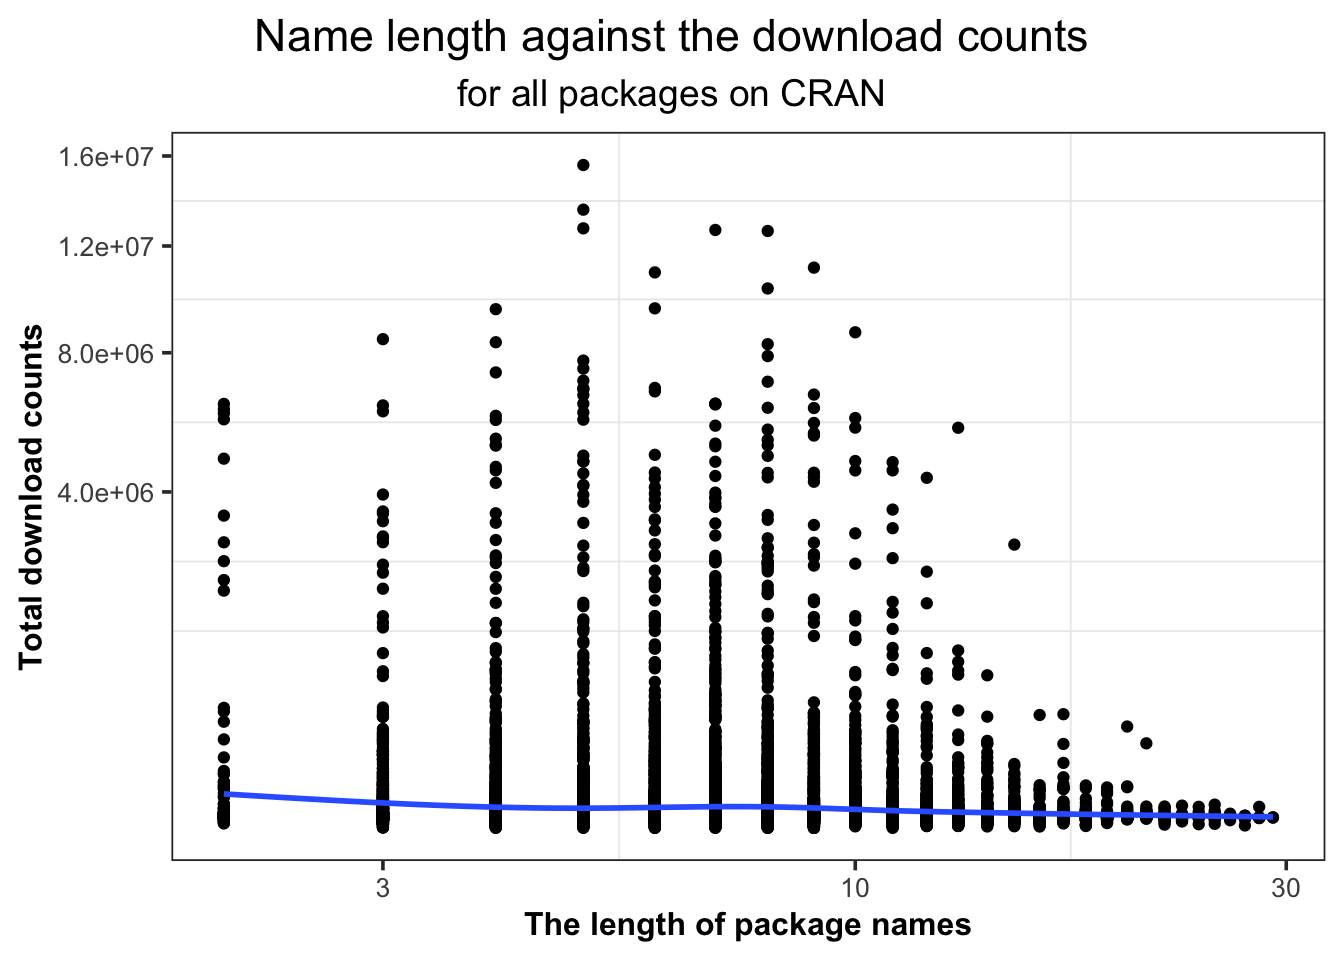
\includegraphics{figures/namelength-plot-1} 

}

\caption{The names of R-packages with more than 6,000,000 downloads are between 5 and 9 characters long.}\label{fig:namelength-plot}
\end{figure}

\begin{discovery}
\textbf{Finding 2}: The average name length of R-packages is about 7.8
characters long, and over half of the R-packages tend to have shorter
names, which may make it more easier to be remembered by users.
\end{discovery}

Table \ref{tab:pct-lngname} shows that the average name length of all the R-packages is 7.8461146. And over half of the CRAN R-packages are more likely with name lengths below average. And R-packages with shorter names can be easier to get relatively higher downloads. That may because shorter named packages are easier for users to remember.

\begin{table}

\caption{\label{tab:pct-lngname}Percentage of packages whose name lengths are below average}
\centering
\begin{tabular}[t]{r|r|r}
\hline
number of short names & percentage of short names & total average name length\\
\hline
9286 & 52.59402 & 7.846115\\
\hline
\end{tabular}
\end{table}

After finding that there is no obvious relationship between the name lengths and the download volume, a new question came up : Can the name lengths of the R-packages be linked to the time of initial release date?

\begin{discovery}
\textbf{Finding 4}: For task view R-packages, the name lengths increase
with the initial release dates, especially for Bayesian packages.
\end{discovery}

We may have this kind of experience in life : for example, detective novels, the later they are released, the less names can be chosen, because many names have been occupied by the books published earlier, with the same theme. Therefore, those later published books often have to lengthen their names to distinguish themselves from the existing books. Coincidentally, we guessed the naming of R-packages from the same topic would also be correlated to the initial release time. So, we looked back to the CRAN task view R-packages\citep{crantaskviews}, for conducting comparison among R-packages from the same topic. Figure \ref{fig:namelth-taskview} shows the name lengths of CRAN task view R-packages against the initial release dates. It is obvious that the name lengths of task view R-package tend to increase with the initial release dates, especially for \texttt{Bayesian} R-packages.



\begin{figure}

{\centering 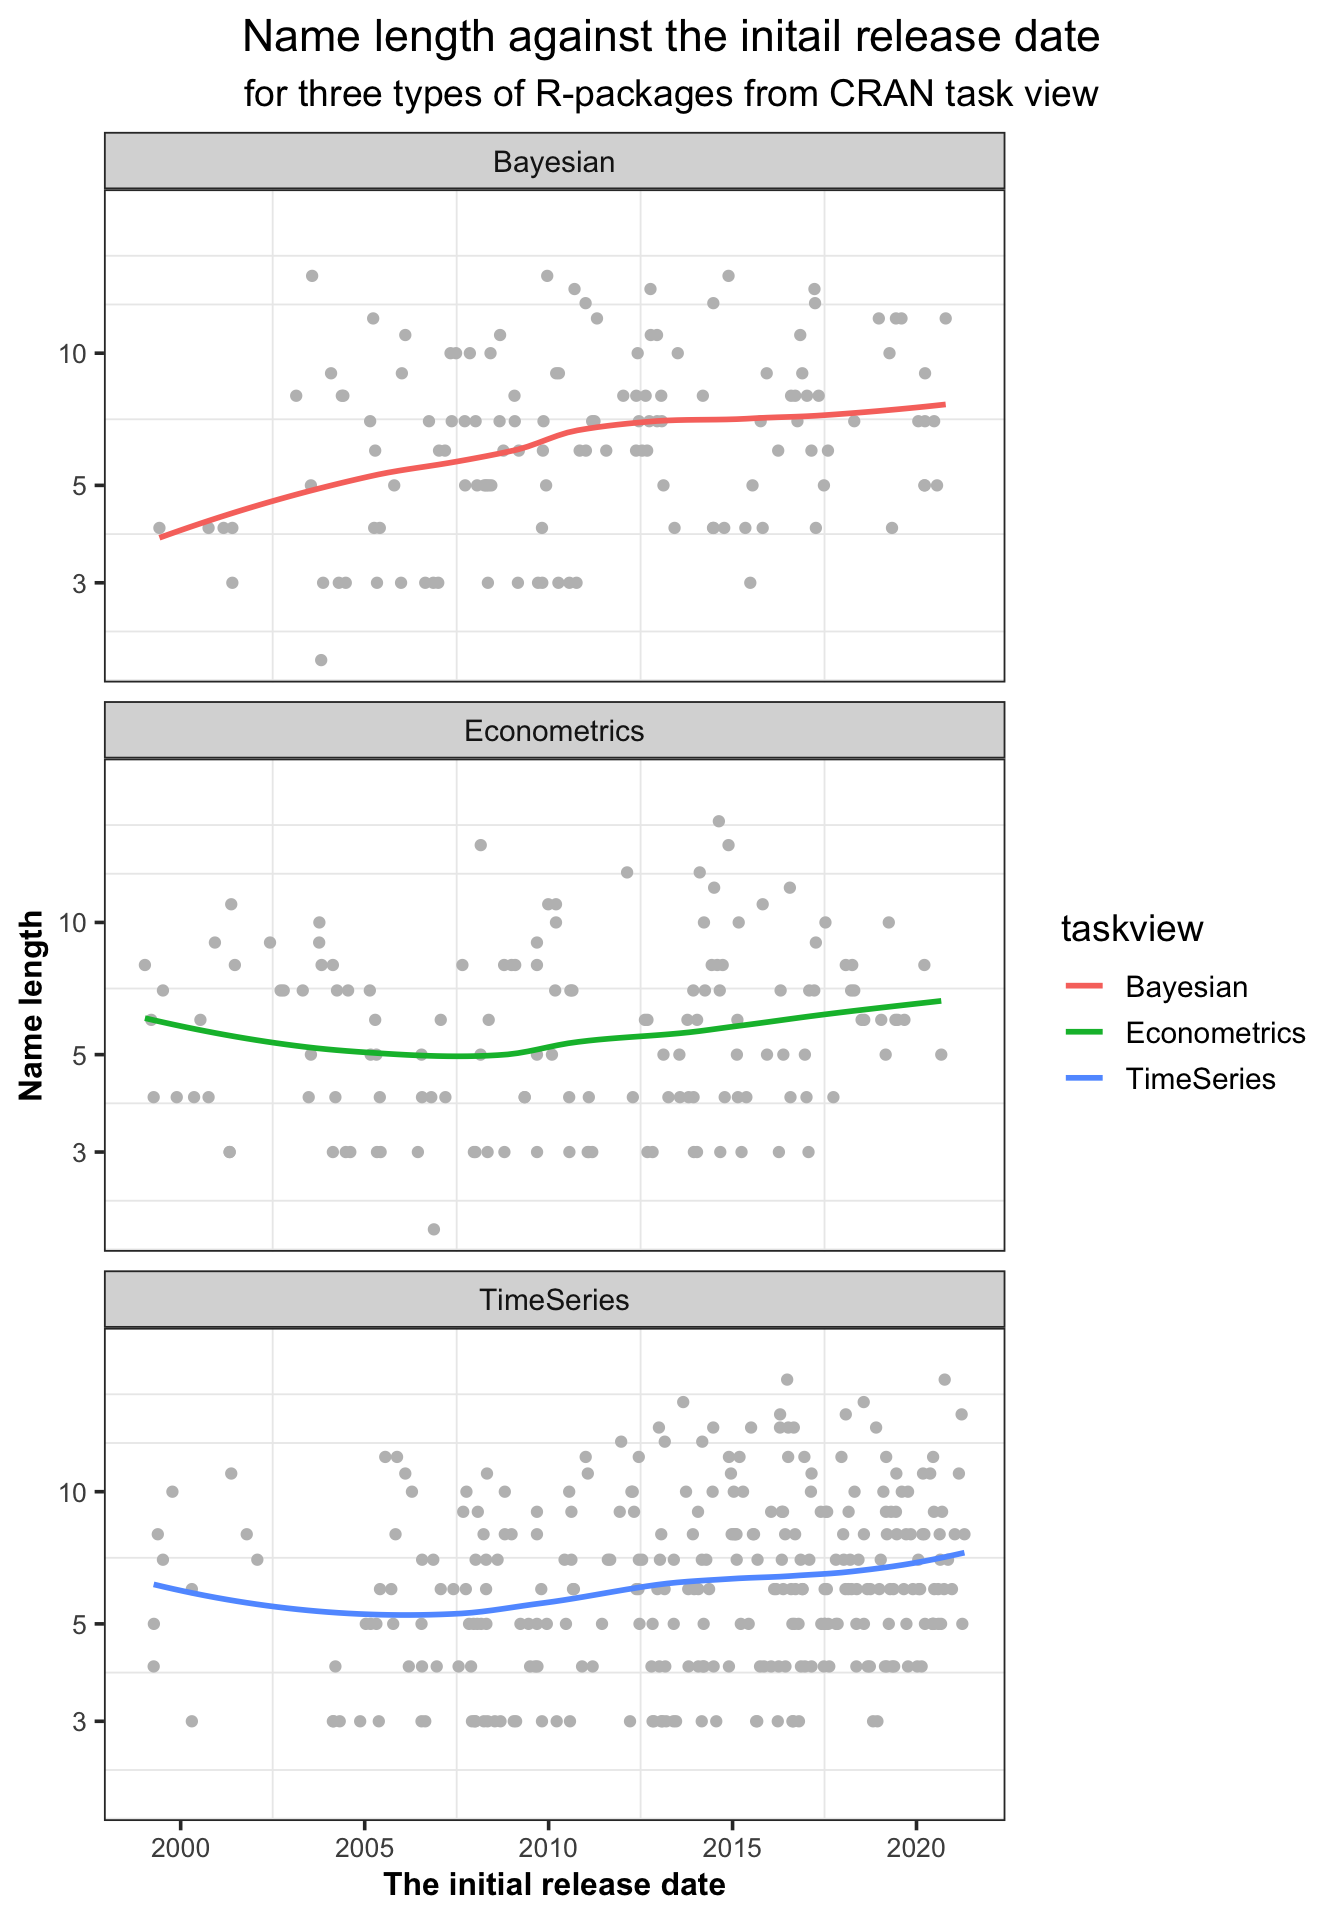
\includegraphics{figures/namelth-taskview-1} 

}

\caption{The name lengths of task view R-packages slightly increase with the initial release dates.}\label{fig:namelth-taskview}
\end{figure}

\begin{discovery}
\textbf{Finding 5}: For all of R-packages on CRAN, the average name
length tends to generally increase with the initial release date.
\end{discovery}

Although we'd better explore this question among R-packages within the same topic, we also had a view on the annual change in the average name length, for all of R-packages on CRAN.

Figure \ref{fig:avgnamelth-year} shows the average name length for all of R-packages on CRAN, released in each year. It is obvious that the name lengths of those R-packages generally increase year by year.



\begin{figure}

{\centering 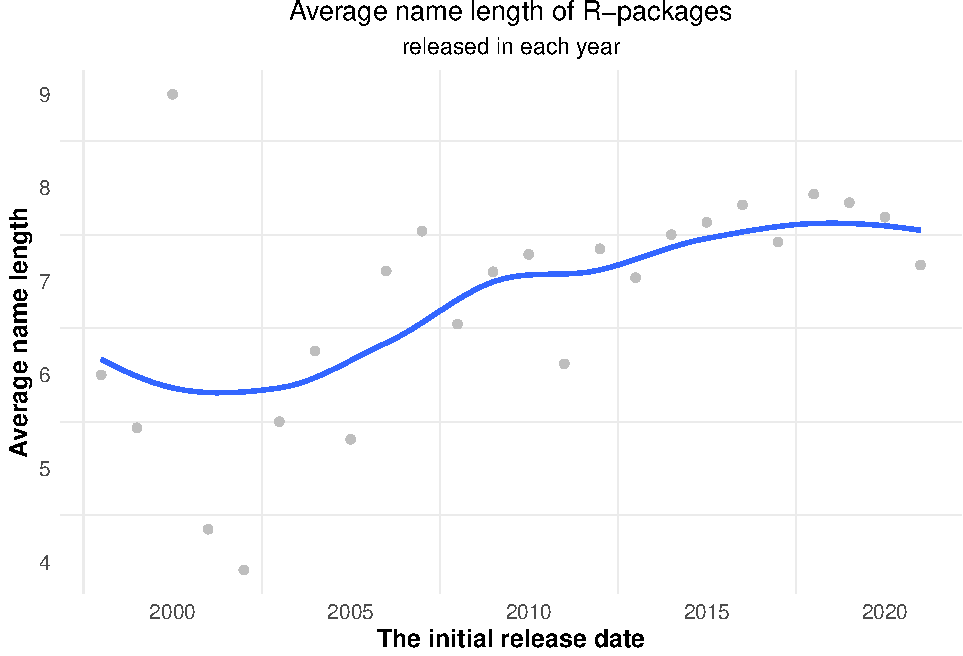
\includegraphics{figures/avgnamelth-year-1} 

}

\caption{The average name length for all of R-packages on CRAN released in each year, tends to rise along the time.}\label{fig:avgnamelth-year}
\end{figure}

\hypertarget{compare-download-counts-with-alphabetical-order-of-names}{%
\section{Compare download counts with alphabetical order of names}\label{compare-download-counts-with-alphabetical-order-of-names}}

We might also have such experiences in our life : when we go shopping in the supermarket, the products placed in front of the shelves can be noticed by us easier. From the perspective of R-packages, in addition to the lengths of names, we also wondered whether alphabetical order can link to the download volume. R-packages with earlier alphabetical order will be placed at the first part of package list on CRAN\citep{cranpkgsname}. To answer this question, we grouped the R-packages by 26-letter order, calculated the average downloads for each group, and made comparisons.

\begin{discovery}
\textbf{Finding 1}: For all of CRAN R-packages, the average downloads of
different alphabetical groups are slightly increasing with alphabetical
order, while the total downloads tend to decrease a little, on the
contrary.
\end{discovery}

From Figure \ref{fig:ahlpha-downloads}, we could see that the average downloads of different alphabetical groups are slightly increasing with alphabetical order, while the total downloads tend to decrease, instead. That is because the later-ordered groups contain fewer R-packages. Developers may prefer to name their packages with top alphabetical order, which might be easier for users to notice.



\begin{figure}

{\centering 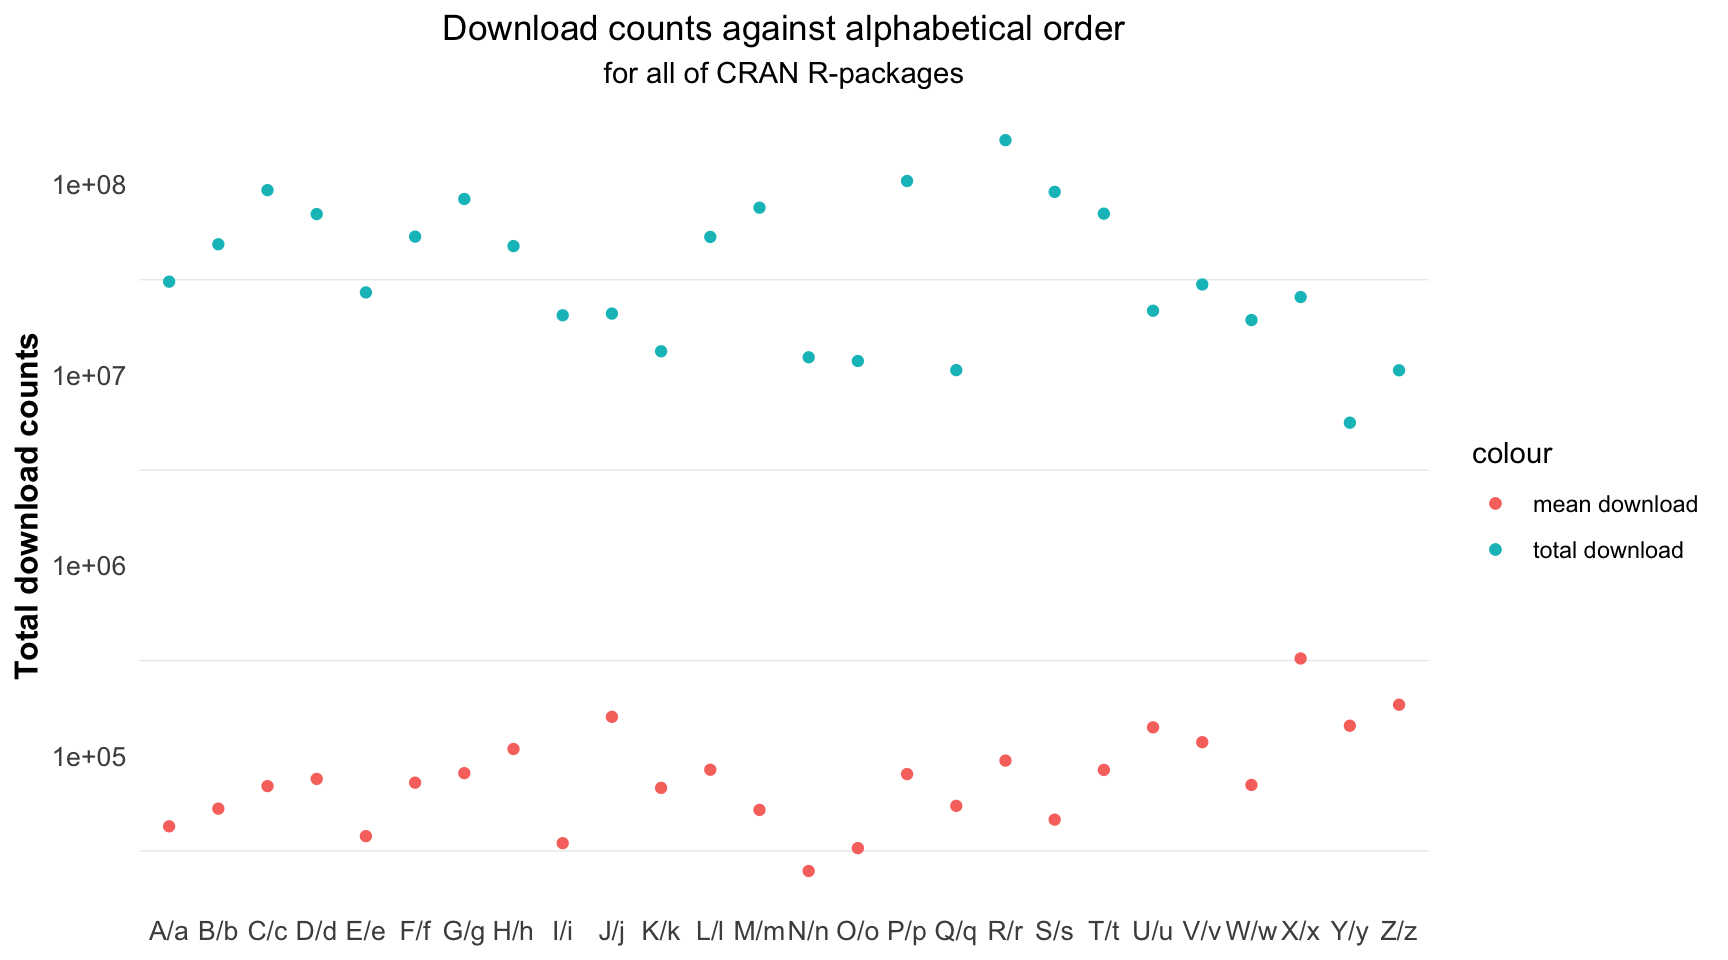
\includegraphics{figures/ahlpha-downloads-1} 

}

\caption{The average total download counts of each group is little linked to the alphabetical order of name, for all of R-packages.}\label{fig:ahlpha-downloads}
\end{figure}

\begin{discovery}
\textbf{Finding 2}: For all of R-packages on CRAN, alphabetical groups
with higher total downloads tend to have greater variance, owing to more
outliers.
\end{discovery}

Then, we took a look at how the variance varies across groups. Figure \ref{fig:all-boxplot} shows the data range and the median value for each alphabetical group. It can be seen that the group ``R/r'' has the highest outlier and the group ``X/x'' has the largest variation. The variances across groups difference little, which means that for each group, 50\% of the download counts are relatively concentrated. The real difference is the highest and lowest downloads per group. In general, the larger the total numbers of downloads (which also means more packages in this group), the more outliers can be included, such as group ``F/f'', ``L/l'' and ``R/r''.



\begin{figure}

{\centering 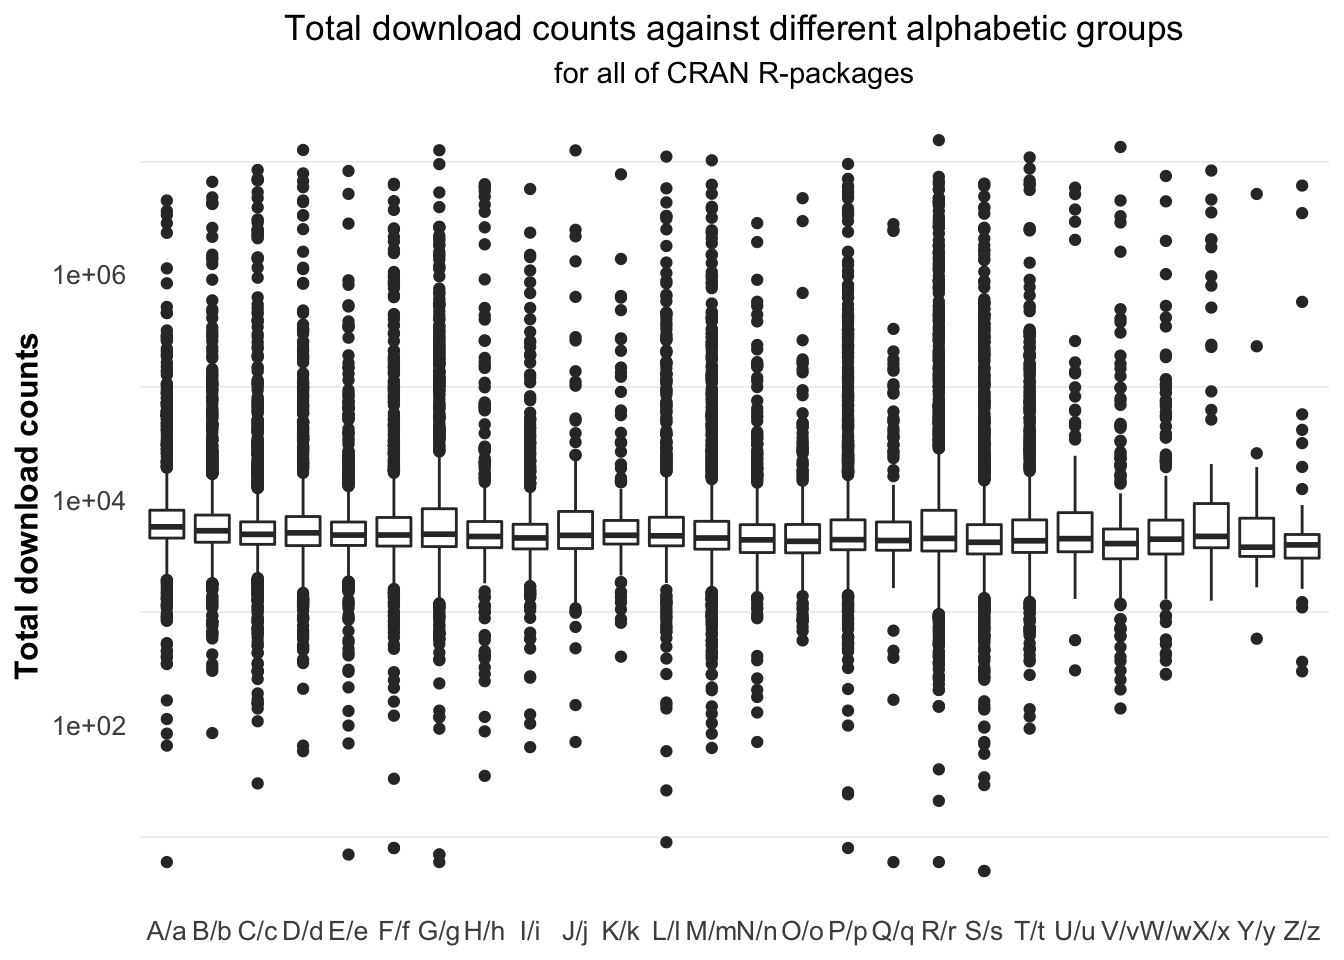
\includegraphics{figures/all-boxplot-1} 

}

\caption{The R-packages with name starting with ``j'' has the largest variation.}\label{fig:all-boxplot}
\end{figure}

In order to further verify our conclusion, we turned to the ultra-low-downloaded R-packages. As mentioned previously, when it comes to the ultra-low-downloaded R-packages, we could approximately assume the only factor that may affect the downloads is name order here.
From Figure \ref{fig:lowdownload-boxplot}, we could see that the difference in median download counts of each alphabetical group is not significant as we expected.



\begin{figure}

{\centering 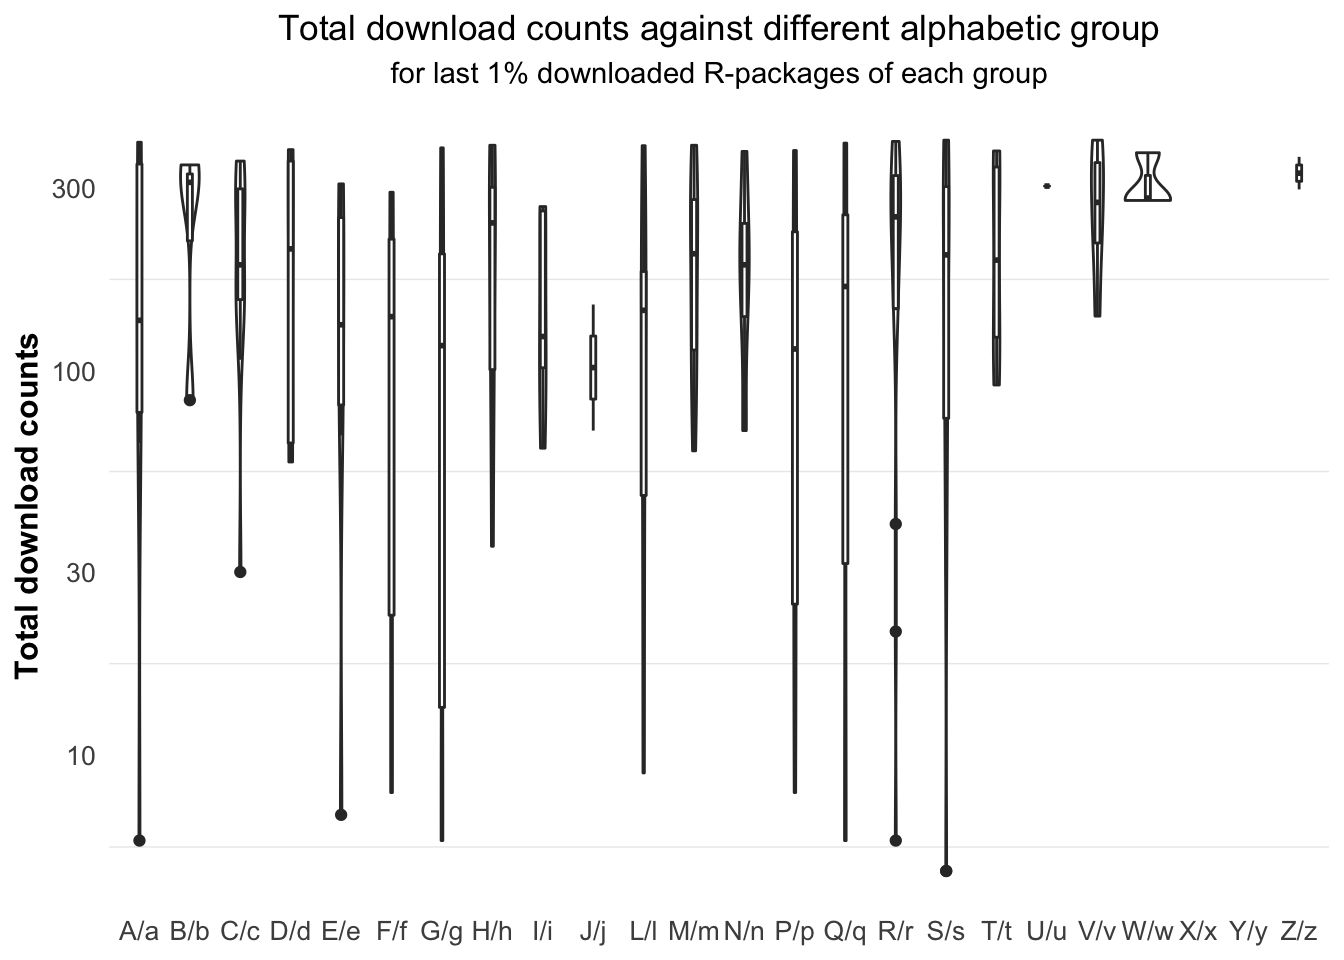
\includegraphics{figures/lowdownload-boxplot-1} 

}

\caption{The last 1\% downloaded R-packages with name starting with ``U/u'' has only one observation.}\label{fig:lowdownload-boxplot}
\end{figure}

Therefore, we could approximately draw a conclusion : In general, the R-packages with top alphabetical order can be easier to get relatively higher download volume, with non-significant gaps. At the same time, the higher the numbers of downloads, the greater the variance can appear in this group.

\hypertarget{summary}{%
\chapter{Summary}\label{summary}}

In this project, we collected summary daily download logs of R-packages through web Application Programming Interface (API) maintained by r-hub\citep{rhub} and also used daily download data in CRAN for a time period from 2012-10-01 to 2021-06-12, to explore the daily download pattern for all of R-packages each year. In that case, we found that the cumulative numbers of downloads increase over time, with an also increasing variance, which indicates that some R-packages with larger downloads grow rapidly. In addition, there is also a strong weekly seasonality in the daily download pattern. The download counts tend to peak through weekdays and drop on weekend. What's more, through Lorenz curve, we also found that most of the cumulative downloads came from the top 10\% downloaded R-packages, which means the distribution of downloads is quite unequal. Part of the reason is that those top 10\% downloaded R-packages contain quite a lot popular and frequently used R-packages, such as \texttt{tidyverse} and \texttt{rlang} that would probably obtain high downloads. In addition, there are other R-packages that often get high download volume, which can be divided into the following four categories:

\begin{itemize}
\tightlist
\item
  R-packages maintained by R studio
\item
  R-packages created by authors from R core group
\item
  R-packages created by authors from R secondary group
\item
  R-packages created by R related authors
\item
  R-packages created by top 20 prolific maintainers (This is resourced at \citet{revolutions})
\end{itemize}

However, the existence of those R-packages may make it difficult to reflect the popularity of other R-packages, so we excluded them, for the analysis of user preferences. And we found that the topics of newly added R-packages on 1st Oct of each year are from quite different application areas, while the R-packages remaining most stably popular during 2017 and 2019 is related to JAVA dependency. Definitely, JAVA always rank top three among programming languages according to TIOBE Index\citep{tiobe}.

As for R itself, its download pattern is quite similar to that of total R-packages on CRAN. The most used OS for R users is windows OS. Also, the most popular version of R is 3.2.1.

After exploration of the characteristics of download pattern for R-package and R, we extracted the release dates for all of CRAN R-packages and task view R-packages, to compare the total download counts (past year for task view R-packages and the most recent 6 month for all) among R-packages with different release dates or with different numbers of updates. And we found that for R-packages from the same topic, earlier release date can usually related to more download counts, while R-packages with more update times would not always have higher downloads. R-packages released earlier and kept being updated are more likely to have higher downloads.

In the next section, we initially tried to scrape the numbers of commits in Github repositories, for all of available CRAN R-packages, through Github API by R, to check whether more commits can result in more downloads. But there came a tricky problem on the rate limit of Github API. As documented in \citet{githubapi}, unauthenticated users could only be permitted to send 60 requests per hour. And only after get authentication, could the rate limit be expanded up to 5000 per hour. However, after trying several methods to get authentication, the rate limit was failed to be promoted. In that case, we switched to make this done with Python by setting random user agent. Meanwhile, in order to display our initial research idea, we still had a look at the last 1\% downloaded R-packages on this question with the original R method. Therefore, we could expect that, generally, if an R-package has more commits on master (main) branch in Github repository, it can probably obtain more download counts.

The last two parts are about analysis for R-package names. We compared the average downloads among R-packages with different name lengths and different alphabetical orders. It is believed that over half of the R-packages tend to have shorter names , probably for the sake of being easily remembered by users. Alphabetical order played little roles in promoting the download volume.

\hypertarget{conclusion}{%
\chapter{Conclusion}\label{conclusion}}

In conclusion, we hold the belief that the download counts can be a relatively simple and reliable measurement for popularity of CRAN R-packages, and there are many factors that could be linked to it, such as the popularity of the creator, the application fields, the release dates, whether to keep updated, and the lengths of their names. Anyway, we could generally believed that a relatively popular R-package should have earlier release date, shorter name and maybe more commits in Github repository if they have. There is also another point that could not be ignored : it is better to keep updated.

  \bibliography{book.bib,packages.bib}

\end{document}
